\documentclass{listhesis}
% --- Listhesis builds on KOMA script report (scrreprt).
%     Class arguments are passed to that class.

% --- Add additional packages here using \usepackage{package-name}.
\usepackage{graphicx}
\graphicspath{{./include/geometry/},
			  {./include/figure_2.0/old/},
			  {./include/figure_2.0/PC_current/},
			  {./include/figure_2.0/PC_new/},
			  {./include/figure_3.5/old/},
			  {./include/figure_3.5/PC_current/},
			  {./include/figure_3.5/PC_new/},
			  {./include/figure_5.0/old/},
			  {./include/figure_5.0/PC_current/},
			  {./include/figure_5.0/PC_new/},
			  {./include/oscillation/},
			  {./include/motivation/}}
\usepackage{afterpage}
\newcommand\blankpage{%
    \null
    \thispagestyle{empty}%
    \addtocounter{page}{0}%
    \newpage}
\usepackage{multirow}
\usepackage{moreverb}
\usepackage{listings}
\usepackage{tcolorbox}
\usepackage{epstopdf}
\definecolor{light-gray}{gray}{0.95}
\definecolorset{RGB}{TUM}{}{%
Black,   0,   0,   0;%
Gray,   51,  51,  51;%
White, 255, 255, 255;%
Blue, 0, 101, 189;%
Ivory,  218, 215, 203;%
Orange, 227, 114,  34;%
Green,  162, 173,   0%
}%
\definecolorset{RGB}{TUMGray}{}{%
Lighter,  128, 128, 128;%
Lightest, 204, 204, 204%
}%
\definecolorset{RGB}{TUMBlue}{}{%
Darkest,    0,  51,  89;%
Darker,     0,  82, 147;%
Lighter,  100, 160, 200;%
Lightest, 152, 198, 234%
}%
\usepackage{amsmath}
\usepackage{amssymb}
\usepackage{amsfonts}
\usepackage{upgreek}
\usepackage{listings}
\lstset{
  basicstyle       = \footnotesize,
  captionpos       = b,
  tabsize          = 4,
  commentstyle     = \color{TUMGreen},
  keywordstyle     = \color{TUMBlue},
  stringstyle      = \color{TUMOrange},
  otherkeywords    = {
    uint64_t,
    uint32_t,
    uint16_t,
    uint8_t,
    u64,
    u32,
    u16,
    u8,
    inline,
    boost::multiprecision::uint128_t
  },
  numbers          = left,
  xleftmargin      = 7ex,
  aboveskip        = 4ex,
  abovecaptionskip = 2ex,
}
\usepackage{siunitx}
\sisetup{
  exponent-product = \cdot,
  %output-product   = \cdot,
  per-mode         = symbol-or-fraction,
  %quotient-mode    = fraction,
  %binary-units     = true
}

% --- Provide your thesis details here.
\setup{%
  de,                   % uncomment if your thesis is in German
  author=Berke Karakin, % your name
  title={Numerische Weiterentwicklung des „ContaminationFlow“
Teilchentransportcodes zur Simulation von
Kontaminationsübertrag in Vakuumanwendungen},
  date={14. März 2022}, % submission date (today is used if unset)
  type=ingenieurpraxis,        % thesis type [master, bachelor, research, internship, diplom]
  advisor=Rudolf Schönmann, % your advisor (typically some PhD. student)
  supervisor=Prof. Dr. rer. nat. habil. Gabriele Schrag, % your supervisor
  % % uncomment the next lines if your thesis was carried out in industry
  % company=External Company,
  % externalAdvisor=Your Companyadvisor
}

\begin{document}

\maketitle
\cleardoublepage
\afterpage{\blankpage}

% --- Thesis abstract.
%     For German thesis also provide an English version via the optional
%     argument: \abstract[English]{German}
%\abstract{An abstract is defined as an abbreviated accurate
%  representation of the contents of a document. -- American National
%  Standards Institute (ANSI)}
%\makeabstract

% --- Content tables.
\tableofcontents
\clearpage
\listoffigures
%\clearpage
\begingroup
\let\clearpage\relax
\listoftables
\endgroup
%\listoftables
%\clearpage

% --- Your thesis starts here.
%     Use \chapter{}, \section{}, \subsection{}, \subsubsection{},
%     and \paragraph{} to structure your thesis.

\chapter{Einleitung} \label{chap:einleitung}
\paragraph{}
Die optischen Instrumente sind das entscheidende Element für die Erdbeobachtungssatelliten in der Erdlaufbahn, die für die optische Fernerkundung eingesetzt sind, bzw. für die Raumsonden, die für die Weltraumforschung eingesetzt sind~\cite{hammar}. Insbesondere spielen die optischen Instrumente der Umweltsatelliten eine wichtige Rolle für die hochauflösende Beobachtung der Erde mittels Bildaufnahme von der Erdoberfläche~\cite{zhang}. Die erhaltenen Daten werden dann in verschiedenen Disziplinen ausgenutzt. 
%\paragraph{}
Jedoch ist es bekannt, dass die Oberflächen der optischen Instrumente der Raumflugkörper empfindlich auf die flüchtigen Substanzen, die eine Kontamination verursachen, reagieren~\cite{jiao}. Der Grund für die Kontamination der Optiken, die nie komplett verhindert werden kann, sind die Wassermoleküle oder die organischen Materialien, die durch die Ausgasung der Satellitenkomponenten entstehen und an den kritischen Oberflächen adsorbieren~\cite{schlappi}. Infolgedessen entsteht an den Oberflächen der optischen Instrumente eine Schicht von unerwünschten Substanzen, die die Leistung des Instruments erniedrigen kann. Diese Kontaminationsschicht kann sogar zum totalen Ausfall des Instruments führen und somit den Ausfall des Satelliten in seiner Laufbahn verursachen~\cite{jiao}.
\paragraph{}
Das Programm „ContaminationFlow“ basiert auf dem Monte-Carlo-Simulator Molflow+, der für die Analyse und für den Entwurf der Hochvakuumsysteme und ihrer Komponenten dient~\cite{molflow}. ContaminationFlow erweitert dieses Programm mit einem Kontaminationsmodell, um die zeitliche Entwicklung der Kontaminationsschicht an den Oberflächen einer Geometrie, in der das Ultrahochvakuum herrscht, durch eine Monte-Carlo-Simulation abzuschätzen. Das Ziel bei der Entwicklung des Programms ist die Schaffung eines Tools zur Vorhersage der Kontamination und die Klassifizierung des Risikos, die bei dem Entwicklungsprozess der optischen Satelliten eingesetzt werden kann~\cite{contaminaton}.
\paragraph{}
Wie es in folgenden Kapiteln detailliert erwähnt wird, berechnet das Programm die Bedeckung der Oberflächen in exponentiell wachsenden Zeitschritten. In bestimmten Fällen führt eine große Schrittweite zur Oszillation der Bedeckung, die dann zu unrealistischen Ergebnissen führt. In dieser Ingenieurpraxis geht es um die Erweiterung des iterativen Algorithmus von ContaminationFlow für die Berechnung der Bedeckung bzw. des Bedeckungsgrads mit dem Prädiktor-Korrektor-Verfahren, um dieses Problem zu verbessern. Das Verfahren ist analog zu dem Heunverfahren, das zur numerischen Lösung eines Anfangswertproblems benutzt wird. Da aber das Programm eigentlich keine Differenzialgleichung integriert, muss das Verfahren anders in den Code implementiert werden. In diesem Bericht wird auf zwei möglichen Ansätze für die Implementierung des Prädiktor-Korrektor-Verfahrens in dem Algorithmus eingegangen. 
\paragraph{}
In Kapitel~\ref{chap:hintergrund} wird ein Hintergrund gegeben, damit das Funktionsprinzip des Programms klar wird. In Kapitel~\ref{chap:durchfuehrung} wird die Implementierung des Prädiktor-Korrektor-Verfahrens beschrieben. Anschließend werden in Kapitel~\ref{chap:auswertung} die neu implementierten Methoden miteinander und gegenüber dem vorherigen Verfahren verglichen und ausgewertet. Letztlich werden in Kapitel~\ref{chap:abschluss} die Ergebnisse zusammengefasst und ein Ausblick wird gegeben.

\chapter{Hintergrund} \label{chap:hintergrund}
\paragraph{}
In diesem Kapitel wird ein Hintergrund zu ContaminationFlow gegeben. Die hier vermittelten Informationen basieren auf der Doktorarbeit von Marton Ady~\cite{marton} sowie auf der Dokumentation von ContaminationFlow.

\section{ContaminationFlow} \label{section:contaminationflow}
\paragraph{}
Das Programm ContaminationFlow basiert auf Molflow+. Molflow+ benutzt die Monte-Carlo-Methode, um die technisch relevanten Größen für die Oberflächen eines beliebig komplizierten Vakuumsystems abzuleiten, deren analytische Berechnung schwer bis unmöglich ist. Als Beispiel zu diesen Größen kann der Druck, die Teilchendichte, die Adsorption, die Desorption sowie die Geschwindigkeit- und Winkelprofilen gegeben werden. Bei der Monte-Carlo-Methode wird nur eine beschränkte Anzahl der Teilchen, die als virtuelle Teilchen oder als Testteilchen bezeichnet wird, betrachtet und ihre Bewegung in einem System, in dem Ultrahochvakuum herrscht (korrespondiert zu einem Druckwert kleiner als \SI{e-7}{\milli\Bar}), simuliert. Unter Anwendung der aus der Simulation erhaltenen Ergebnisse wird eine Abschätzung für die oben genannten technischen Größen gemacht. Übrigens, weil es in dem System Ultrahochvakuum herrscht, ist die mittlere freie Weglänge der Teilchen viel größer als die Größe der Geometrie. Das heißt, es herrscht näherungsweise die freie molekulare Strömung im Inneren des Systems. Als Konsequenz kann vereinfacht angenommen werden, dass einzelne Teilchen nicht mit anderen Teilchen in dem System stoßen, was unter normalem Druck sehr wahrscheinlich wäre. Diese Annahme erlaubt die Parallelisierung der Simulation, weil die simulierten Testteilchen während ihrer Flugzeit nur mit den Oberflächen der Geometrie wechselwirken. Außerdem ist die Simulation ereignisgesteuert. Das heißt, die physikalische Zeit in dem System vergeht nur nach bestimmten Ereignissen, wie zum Beispiel der Stoß mit einer Oberfläche. 

\begin{figure}[]
\centering
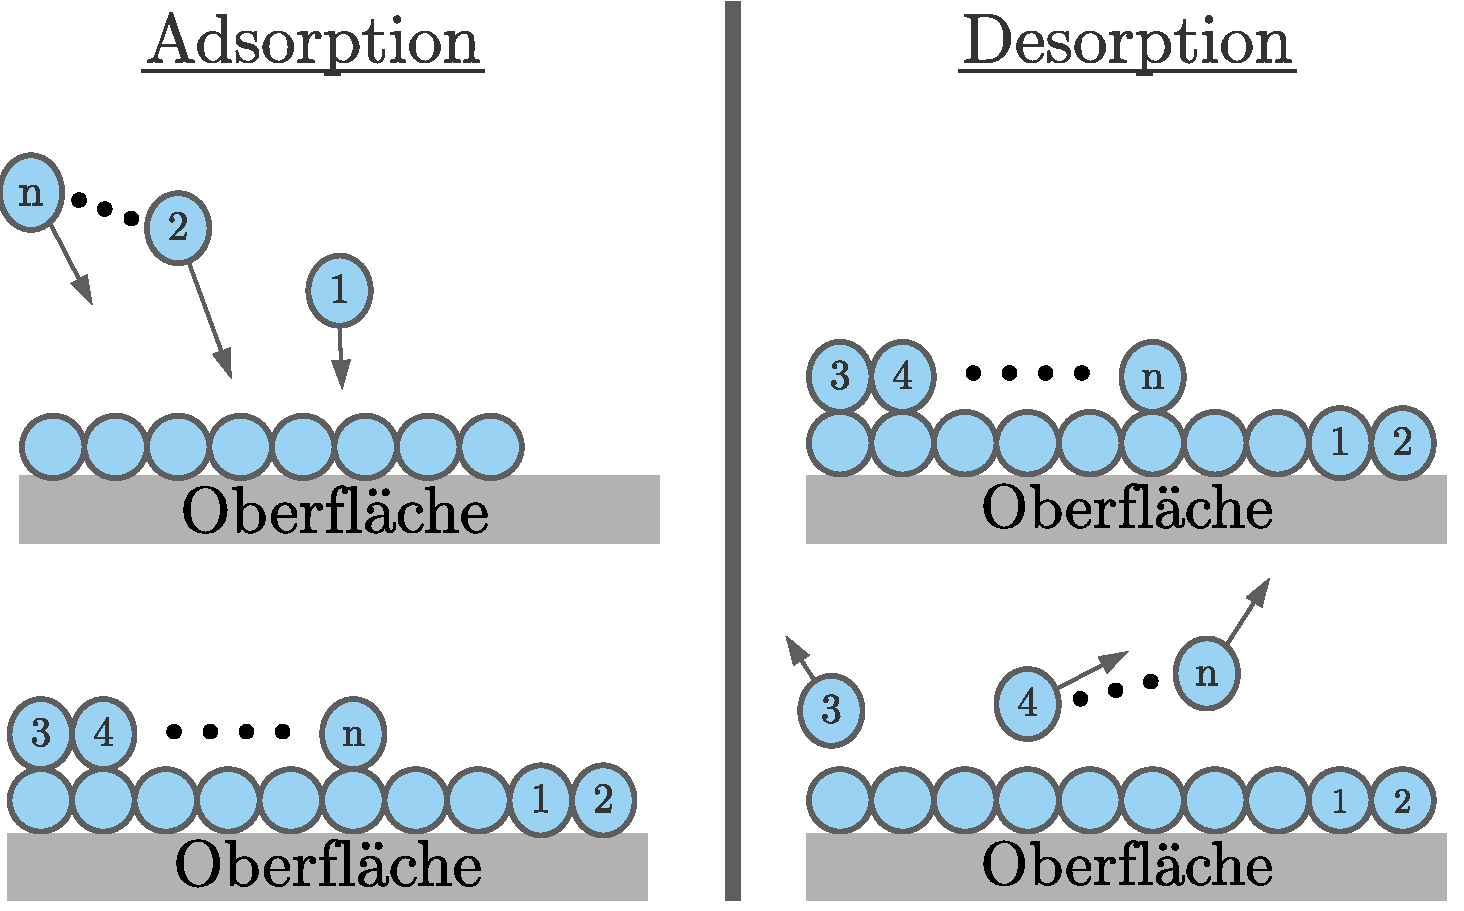
\includegraphics[width=0.55\textwidth]{adsorption_desorption.pdf}
\caption{Kontaminationsmodell}
\label{fig:model}
\end{figure}

\paragraph{}
ContaminationFlow erweitert Molfow+ mit einem Kontaminationsmodell, um die Kontamination an den kritischen Oberflächen der Satelliten abschätzen zu können. Infolgedessen wird zu den oben genannten relevanten Größen auch die Bedeckung ($\theta^*$) bzw. der Bedeckungsgrad ($\theta$) hinzugefügt. Mit der Bedeckung wird die Anzahl der Teilchen, die sich an einer Oberfläche der Geometrie befinden, ausgedrückt bzw. mit dem Bedeckungsgrad wird die Anzahl der Schichten, die die Teilchen an einer Oberfläche bilden, ausgedrückt. Für die Modellierung der Kontamination wird eine Vereinfachung gemacht und es wird davon ausgegangen, dass alle Teilchen, die an einer Oberfläche adsorbieren, zuerst eine Kontaminationsschicht komplett füllen, bevor sie mit der nächsten Schicht weitermachen. Im Falle der Desorption können zuerst die obersten Teilchen desorbieren. Dieser Fall wird in der Abbildung~\ref{fig:model} illustriert. Die Satelliten können in ihrer Laufbahn für mehrere Jahre tätig sein~\cite{jiao}. Aus diesem Grund muss das Programm eine physikalische Zeit von mehreren Jahren simulieren. Um diese Simulation rechnerisch zu ermöglichen, werden die Zeitschritte exponentiell wachsend gewählt. Das Programm benutzt mehrere Prozesse. Somit können innerhalb der gleichen Rechenzeit mehr Testteilchen simuliert werden. Da die Monte-Carlo-Methode ein stochastisches Verfahren ist, wird die Genauigkeit der Ergebnisse mit der zunehmenden Anzahl der simulierten Testteilchen auch zunehmen~\cite{fenrg}. Die Prozesse in dem Programm werden in Hauptprozess und Subprozesse unterteilt. Die $K$ verschiedenen Subprozesse sind für die Simulation der Testteilchen zuständig. Sie benutzen keine gemeinsamen Variablen, das heißt, dass jeder Subprozess eine andere Kopie des Programms durchführt. Während der Simulation der Testteilchen in den Subprozessen werden bestimmten Zählern je nach dem geschehenen Ereignis gezählt. Diese Zähler werden dann für die Berechnung der physikalischen Größen gemäß den entsprechenden Formeln, die hier nicht erwähnt werden, zum Hauptprozess geschickt. Es soll beachtet werden, dass in den Subprozessen im Allgemeinen nicht so viele Teilchen, wie sie sich in einem realen System befinden, simuliert werden können. Deswegen wird angenommen, dass jedes simulierte Teilchen mehrere realen Teilchen darstellt. Der Faktor, der dieses Verhältnis beschreibt, wird $K_{real/virtual}$ genannt. Am Ende der Subprozesssimulationen werden ihre Zählerwerte mit diesem Faktor multipliziert, um auf dem realen Ergebnis zu kommen. Der Hauptprozess dient für die Steuerung des Programms sowie für die Akkumulation (Summierung) der in den Subprozesssimulationen erhaltenen Zählerwerte. Am Anfang des Programms werden die Anfangsbedeckungen sowie die Geometrieparameter von dem Hauptprozess zu den Subprozessen geschickt. Am Ende der Subprozesssimulationen werden die erhaltenen Zählerwerte mit dem Faktor $K_{real/virtual}$ skaliert. Danach wird der tatsächliche Wert der oben genannten physikalischen Größen für den nächsten Zeitpunkt berechnet. Im Falle der Bedeckung wird der Zählerwert zuerst vom Zählerwert am Anfang des Zeitschritts subtrahiert und diese Differenz wird mit dem Faktor skaliert. Letztlich wird die skalierte Differenz zur Bedeckung am Anfang des Zeitschritts addiert. Schließlich werden die Subprozessen mit den neu berechneten Größen aktualisiert und das Programm macht mit der nächsten Iteration weiter.

\begin{figure}[t]
\centering
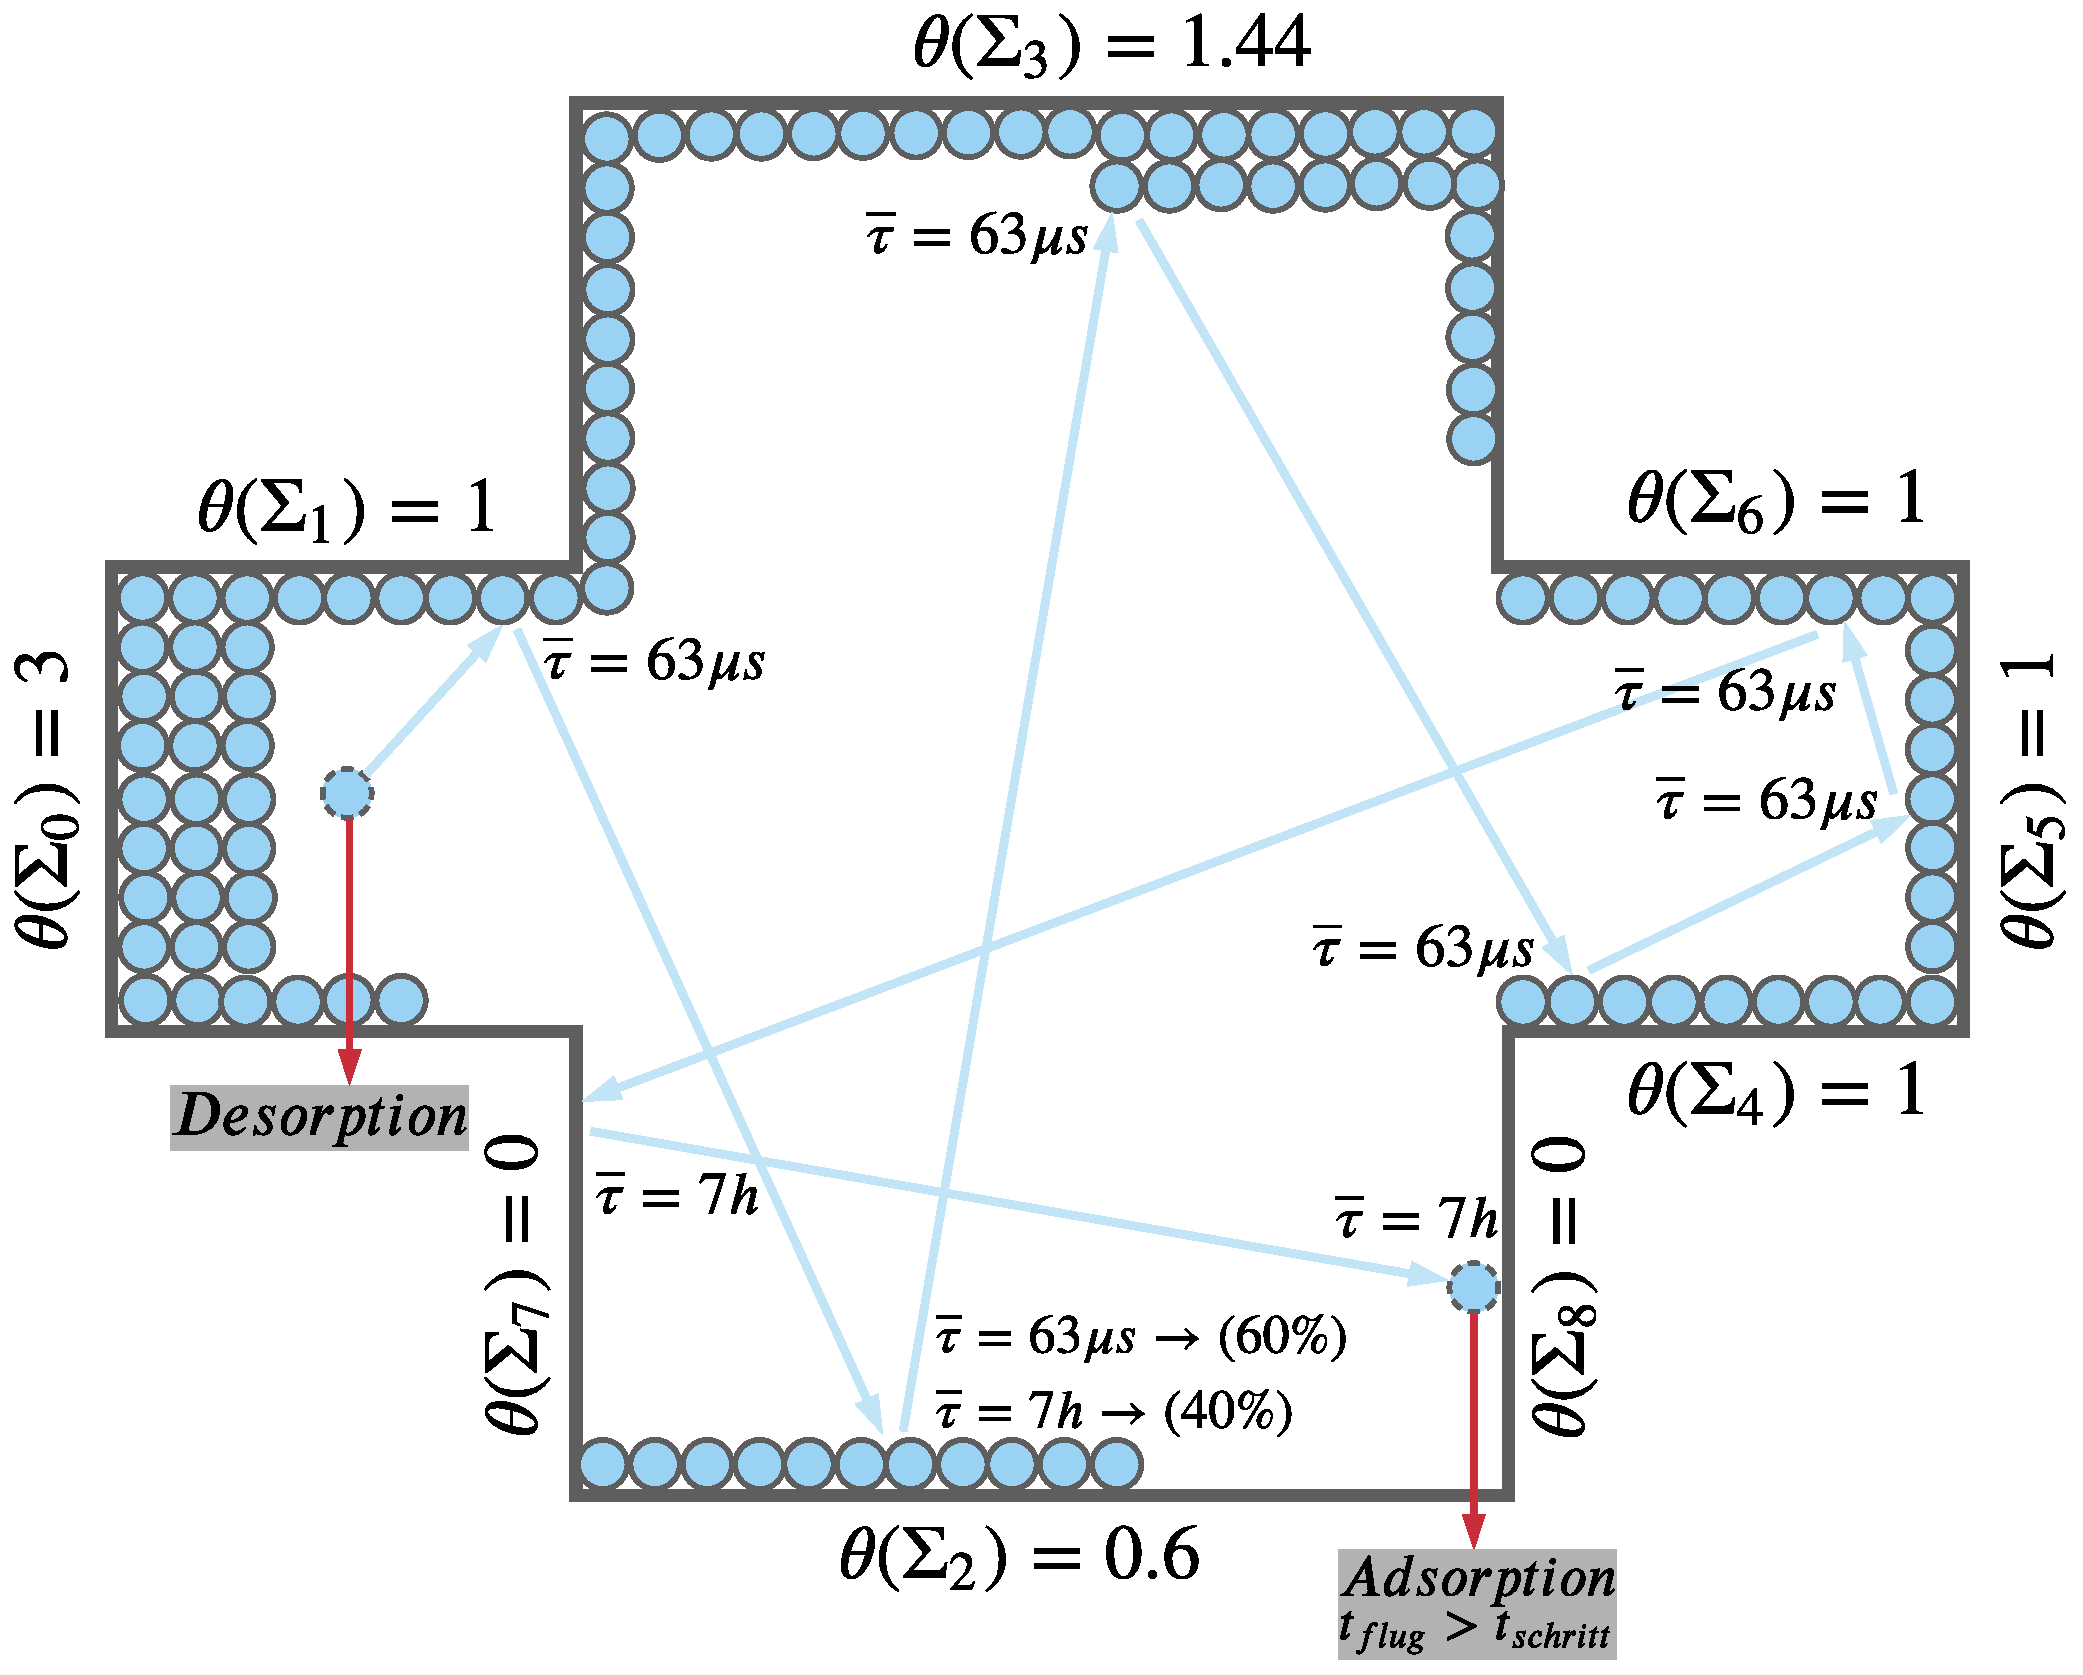
\includegraphics[width=0.655\textwidth]{molecular_flow.pdf}
\caption{Simulation eines Testteilchens in einem Subprozess}
\label{fig:simulation}
\end{figure}

\section{Simulation eines Testteilchens} \label{section:molflow}
\paragraph{}
In der Abbildung~\ref{fig:simulation} wird die Simulation eines Testteilchens für eine Schrittweite von 10 Stunden grob skizziert. Dabei wurden die Geometrie und ihre Bedeckungsgrade beispielhaft gewählt. Am Anfang wird ein Testteilchen in einer zufällig gewählten Oberfläche (in der Abbildung ist sie die Oberfläche $\Sigma_0$) generiert. Die Wahrscheinlichkeit für das Wählen einer bestimmten Oberfläche hängt von ihrer Desorption, die von ihrer Bedeckung abhängt, und von ihrer Ausgasung ab. Nach der Wahl der Oberfläche wird der Startpunkt des Testteilchens an dieser Oberfläche ausgesucht. Die Zufallsvariablen für das Aussuchen eines Startpunkts sind gleichverteilt. Das heißt, jeder Punkt kann mit gleicher Wahrscheinlichkeit gewählt werden. Anschließend wird abhängig von der Desorption und von der Ausgasung der gewählten Oberfläche zufällig entschieden, ob das generierte Testteilchen durch Ausgasung oder durch Desorption entsteht. Diese Unterscheidung ist wichtig, denn im Falle einer Desorption wird davon ausgegangen, dass das Testteilchen aus der Kontaminationsschicht stammt und der Zähler für die Bedeckung der Oberfläche wird um eins erniedrigt. Im Falle der Ausgasung wird angenommen, dass das Teilchen außerhalb des Systems stammt und der Zähler für die Bedeckung bleibt gleich. Nach dieser Unterscheidung wird noch die Verweilzeit des Testteilchens an der Oberfläche zu seiner gesamten Flugzeit addiert und damit die Startzeit des Teilchens bestimmt. In diesem Bericht wird auf die Berechnung der Startzeit nicht eingegangen, weil sie komplex ist. Jedoch kann angenommen werden, dass für einen Bedeckungsgrad größer als zwei jedes desorbierende Teilchen an dem Adsorbat gebunden ist. Damit berechnet sich die Startzeit mit einer kurzen Verweilzeit. Wenn der Bedeckungsgrad kleiner als eins ist, wird angenommen, dass jedes desorbierende Teilchen an dem Adsorbens gebunden ist. Damit berechnet sich die Startzeit mit einer langen Verweilzeit. Ansonsten wird zufällig entschieden, ob das desorbierende Teilchen an dem Adsorbens oder an dem Adsorbat gebunden ist. Denn bei einem Bedeckungsgrad zwischen eins und zwei sind die beiden Bindungstypen des desorbierenden Teilchen möglich. Letztlich wird die Richtung des Testteilchens nach dem Knudsen-Kosinus-Gesetz und die Geschwindigkeit des Teilchens nach der Maxwell-Boltzmann-Verteilung zufällig entschieden. Als Nächstes findet der Raytracing-Algorithmus die nächste Oberfläche, an der das Testteilchen stoßen wird. Die Zeit, die unterwegs vergeht, wird zu der Flugzeit des Testteilchens addiert. Nach dem Stoß an der Oberfläche verweilt das Testteilchen für eine bestimmte Zeit. Wie es in der Abbildung gezeigt wird, hängt die Verweilzeit von dem Bedeckungsgrad der Oberfläche ab. Bei einem Bedeckungsgrad größer als eins bindet das Testteilchen an dem Adsorbat. Dagegen wird bei einem Bedeckungsgrad kleiner als eins zufällig entschieden, ob das Teilchen an dem Adsorbens oder an dem Adsorbat bindet. Wenn das Testteilchen direkt an dem Adsorbens bindet, dann wird die Bindungsenergie zwischen dem Adsorbens und dem Teilchen ($E_{de}$) als die Aktivierungsenergie benutzt. Im Falle der Bindung zwischen einem Wassermolekül und Edelstahl korrespondiert ihre Bindungsenergie (\SI{1}{\electronvolt})~\cite{grinham} bei einer Temperatur von \SI{20}{\celsius} zu einer mittleren Verweilzeit ($\bar{\tau}$) von ca. \SI{7}{Stunden}. Für kurze Schrittweiten wäre die Annahme, dass das Testteilchen an der Oberfläche stecken bleibt, nicht falsch. Anderseits, falls das Testteilchen an dem Adsorbat bindet, dann wird die Verdampfungsenthalpie ($H_{vap}$) als die Aktivierungsenergie benutzt. Im Falle einer Bindung zwischen zwei Wassermolekülen, korrespondiert ihre Bindungsenergie (\SI{0.5}{\electronvolt})~\cite{grinham} bei einer Temperatur von \SI{20}{\celsius} zu einer mittleren Verweilzeit von ca. \SI{63}{\micro\s}. Das heißt, dass das Testteilchen nach einer sehr kurzen Zeit wieder frei wird. Nach dem Addieren der Verweilzeit zu der Flugzeit des Testteilchens werden wieder seine Richtung und seine Geschwindigkeit entschieden. Der gleiche Prozess wiederholt sich, bis die Flugzeit des Testteilchens größer als die Schrittweite ist. In diesem Fall endet seine Simulation. Für den nächsten Zeitpunkt adsorbiert es an der Oberfläche, an der es gerade befindet (in der Abbildung ist sie die Oberfläche $\Sigma_8$) und der Zähler für die Bedeckung dieser Oberfläche erhöht um eins. Anschließend wird mit der Simulation eines anderen Testteilchens weitergemacht, bis es genug Testteilchen simuliert wurden.

\chapter{Durchführung} \label{chap:durchfuehrung}
\paragraph{}
In diesem Kapitel geht es um die Implementierung des Prädiktor-Korrektor-Verfa\-hrens in den Simulationscode. Zuerst wird auf das Oszillationsproblem der Simulationsergebnisse eingegangen. Danach wird die Motivation für die Wahl des Prädiktor-Korrektor-Verfahrens erklärt. Diesbezüglich werden das explizite Eulerverfahren und das Heunverfahren, die zur numerischen Lösung eines Anfangswertproblems verwendet werden können~\cite{ulbrich}, miteinander verglichen. Schließlich wird die tatsächliche Implementierung des Prädiktor-Korrektor-Verfahrens in den Simulationscode beschrieben. Dazu wird auf zwei verschiedenen Ansätzen eingegangen.

\section{Oszillation der Simulationsergebnisse} \label{section:oscillation}

\begin{figure}[]
\centering
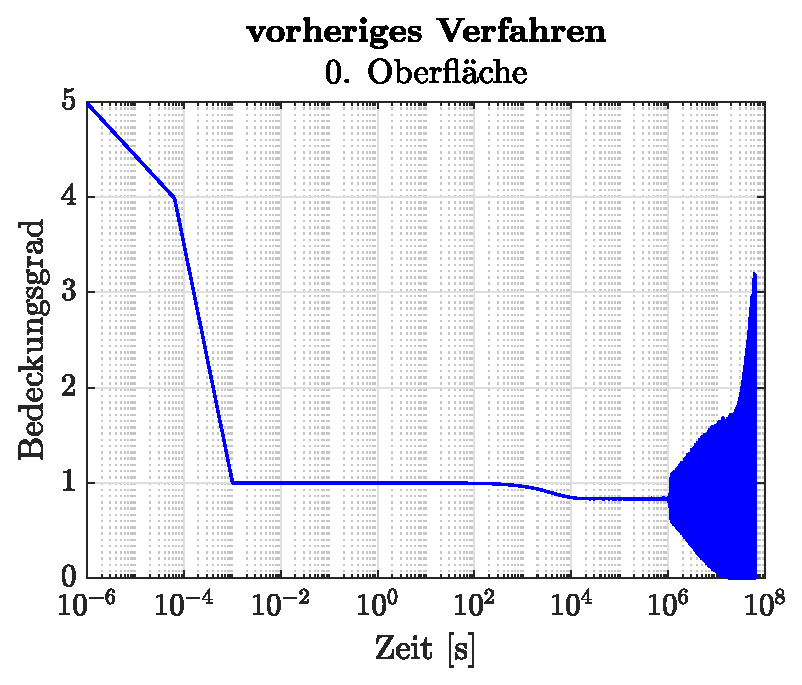
\includegraphics[width=0.5\textwidth]{./include/figure_5.0/old/CovFacet0.eps} 
\caption{Oszillation bei größeren Schrittweiten}
\label{fig:oscillation}
\end{figure}

\paragraph{}
Für die Darstellung des Oszillationsproblems wird eine einfache Würfelgeometrie betrachtet, wobei der Anfangsbedeckungsgrad der 0. Oberfläche 5.0 ist und die Anfangsbedeckungsgrade der anderen Oberflächen 0 sind. Es wird mindestens \SI{e4}{} Testteilchen simuliert. Außerdem gasen keine Teilchen aus den Oberflächen aus. In diesem Fall ist zu erwarten, dass die Bedeckungsgrade aller Oberflächen im Gleichgewicht auf $0.8\overline{3}$ annähern. Dieser Fall ist in der Abbildung~\ref{fig:oscillation}~auf~der~Seite~\pageref{fig:oscillation} zu sehen. Die Abbildung zeigt den Bedeckungsgrad der 0. Oberfläche abhängig von der Zeit. Hierbei wird eine logarithmische Zeitachse gewählt und die Simulation wird für zwei Jahren mit 1000 Iterationen ausgeführt. Daneben wird auf die zeitabhängigen Bedeckungsgrade der anderen Oberflächen nicht eingegangen, weil sie im Gleichgewicht analog zur 0. Oberfläche sind. Die Abbildung zeigt, dass ab dem Zeitpunkt \SI{e6}{\s}, der zum 12. Tag des simulierten Systems korrespondiert, der Bedeckungsgrad stark oszilliert. Dieses Verhalten ist unphysikalisch. Die Schrittweite in diesem Zeitpunkt beträgt ungefähr 3 Stunden. Die Ursache für dieses Verhalten ist nicht einfach zu erklären. Die einfachste Begründung wäre, dass die Monte-Carlo-Methode seine Ursache war, weil sie ein stochastisches Verfahren ist und die Ergebnisse immer eine Ungenauigkeit enthalten. Da am Ende der Subprozesssimulationen die Ergebnisse noch mit dem Faktor $K_{real/virtual}$ skaliert werden, werden auch die Ungenauigkeiten mitskaliert. Aus diesem Grund ist zu überlegen, dass diese Sache der Anlass der Oszillation ist. Aber in diesem Fall ist zu erwarten, dass das Problem mit der Zunahme der Stichprobe gelöst wird. Jedoch passiert das tatsächlich nicht. In der Tat bleibt der Fehler in der gleichen Größenordnung, wenn die Anzahl der simulierten Testteilchen verzehnfacht (\SI{e5} {Testteilchen}) oder verhundertfacht (\SI{e6}{Testteilchen}) wird. Diese Angelegenheit legt die Vermutung nahe, dass es ein Effekt gibt, die die homogene Verteilung der Testteilchen in dem System verhindert. In dem betrachteten Beispiel kann davon ausgegangen werden, dass die Schrittweite in dem Zeitpunkt des Oszillationsbeginns so lang ist, dass ungefähr alle Teilchen an den Oberflächen desorbieren. Wenn aber eine Oberfläche wegen der statistischen Ungenauigkeiten ein bisschen größere Bedeckung hat, dann adsorbiert sie weniger Teilchen. Wogegen, wenn eine Oberfläche ein bisschen niedrigere Bedeckung hat, dann adsorbiert sie mehr Teilchen. In großen Schrittweiten führt diese Asymmetrie irgendwie zu einem selbstverstärkenden Effekt, sodass das in der Abbildung illustrierte Verhalten beobachtet wird. Übrigens ist es möglich, dass die Bedeckung wegen der Oszillation negativ ist. In diesem Fall wird die negative Bedeckung mit 0 ersetzt. Das führt zur Zunahme der Gesamtteilchenzahl in dem System. Die Zunahme der Gesamtteilchenzahl kann mit der Erhöhung der Anzahl der Testteilchen verlangsamt werden.

\section{Motivation für das Prädiktor-Korrektor-Verfahren} \label{section:PK}

\begin{figure}[!h]
\centering
\begin{tabular}{@{}cc@{}}
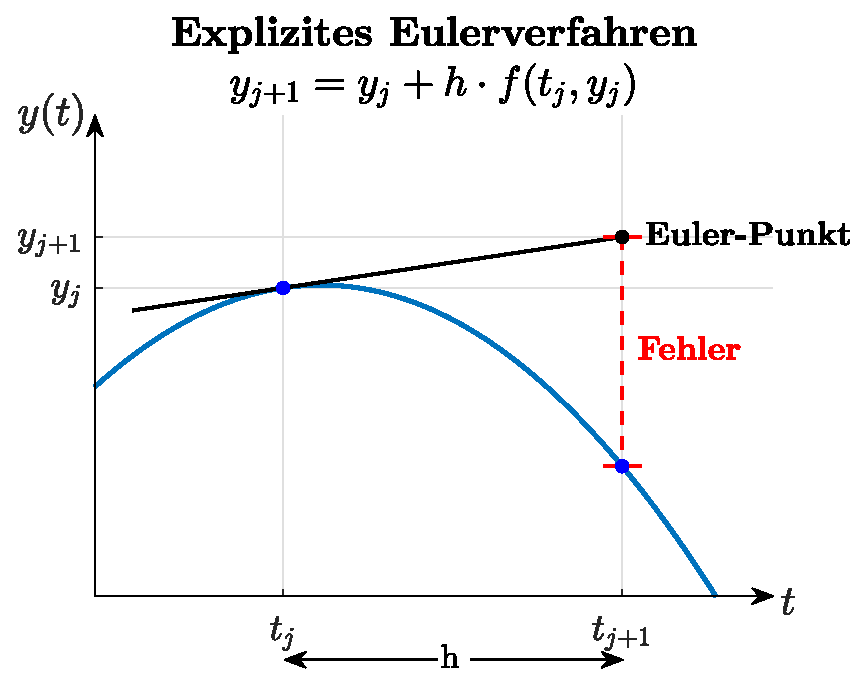
\includegraphics[height=4.7cm, width=0.45\textwidth]{euler}&
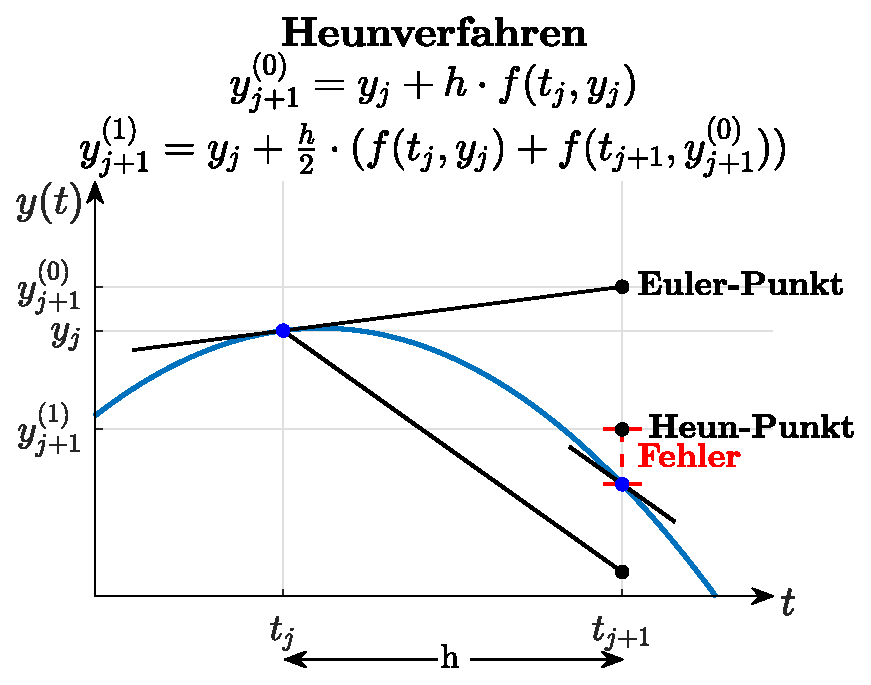
\includegraphics[width=0.45\textwidth]{heun}
\end{tabular}
\caption{Vergleich vom expliziten Eulerverfahren und Heunverfahren}
\label{fig:motivation}
\end{figure}

\paragraph{}
Betrachtet wird ein Anfangswertproblem in der Form:
\begin{gather*}
y'(t) = f(t,y(t))\\ y(t_0) = y_0\: \text{und}\: y:\mathbb{R}\rightarrow\mathbb{R}
\end{gather*}
Die Abbildung~\ref{fig:motivation} zeigt die zwei verschiedenen Algorithmen, die zur numerischen Lösung des oben gezeigten Anfangswertproblems benutzt werden können, und deren Anwendung auf einer Beispielfunktion. Die Verfahren approximieren die Funktion in den diskreten Zeitpunkten. Der linke Graph illustriert die Anwendung des expliziten Eulerverfahrens für einen Schritt und dabei entstandener Diskretisierungsfehler. Zudem ist der Punkt ($t_j,y_j$), was in dem letzten Schritt berechnet wurde. Es wird davon ausgegangen, dass das Verfahren in dem letzten Schritt eine perfekte Approximation ($e_j = |y(t_j) - y_j| = 0$) machte. Außerdem wird die Schrittweite $h$ trotz der schnellen Dynamik der Funktion groß gewählt. Bei dem Eulerverfahren wird die Approximation für den nächsten Schritt ($t_{j+1}, y_{j+1}$) unter Anwendung der im linken Graph gezeigten Formel berechnet. Die Formel kann geometrisch so interpretiert werden, dass aus $f(t,y(t))$ die Steigung der Funktion in dem Punkt ($t_j, y_j$) berechnet wird. Diese Steigung wird dann bis zum nächsten Zeitpunkt gefolgt und der Wert der Funktion in diesem Zeitpunkt mit dem y-Wert des erreichten Punkts approximiert. In dem rechten Graph wird die Anwendung des Heunverfahrens (Prädiktor-Korrektor-Verfahren mit einem Korrektor-Schritt) für einen Schritt und der dabei entstandener Diskretisierungsfehler dargestellt. Die Formel, die im rechten Graph gezeigt ist, kann geometrisch unterschiedlich interpretiert werden. Eine dieser Interpretationen, auf der die Implementierung des Verfahrens in den Simulationscode basiert, wäre, dass es zuerst das explizite Eulerverfahren verwendet wird. Der Punkt, der dadurch erreicht wird, wird für die Approximation der Steigung der Funktion in dem nächsten Zeitpunkt benutzt. Dieser Schritt wird als Prädiktor-Schritt genannt. Da das Eulerverfahren Fehler enthält, weicht die berechnete Steigung von der tatsächlichen Steigung ab. Aus diesem Grund entspricht die Gerade, die durch den Punkt ($t_{j+1},y(t_{j+1})$) geht, keine genaue Tangente. In dem Korrektor-Schritt wird die neu berechnete Steigung vom Ausgangspunkt bis zum nächsten Zeitpunkt gefolgt. Schließlich werden die y-Werte von dem erreichten Punkt und der Punkt aus dem Eulerschritt gemittelt und der Wert der Funktion in dem nächsten Zeitpunkt mit dem y-Wert des neuen Punkts approximiert. Es können auch mehrere Korrektor-Schritte ausgeführt werden, um die Genauigkeit des Verfahrens zu verbessern~\cite{butcher}. In der Abbildung ist zu merken, dass bei dem Heunverfahren der Approximationswert in zwei Schritten berechnet wird. Zwar ist die Rechenzeit dadurch länger, aber der Fehler, der bei der Approximation entsteht, ist deutlich kleiner. Demgegenüber ist der Fehler, der bei dem expliziten Eulerverfahren entsteht, viel größer. Wenn trotz dieses Fehlers mit dem Verfahren weitergemacht würde, dann wäre es sehr wahrscheinlich, dass der Fehler in den nächsten Zeitpunkten immer größer wird. Das bedeutet, dass das Verfahren mit wachsender Amplitude oszilliert und unvernünftige Ergebnisse gibt. Obwohl das Heunverfahren im Allgemeinen bessere Ergebnisse liefert, ist es nicht garantiert, dass es immer so sein wird. Es können auch Anfangswertprobleme konstruiert werden, für die das explizite Eulerverfahren besser geeignet ist. Jedoch ist es garantiert, dass der Fehler des Heunverfahrens quadratisch abnimmt ($\mathcal{O}(h^2)$), wenn die Schrittweite verkleinert wird. Dagegen nimmt der Fehler des Eulerverfahrens mit der abnehmenden Schrittweite nur linear ab ($\mathcal{O}(h)$)~\cite{ulbrich}.

\section{Implementierung} 
\label{section:implement}
\paragraph{}
Im Abschnitt~\ref{section:PK} wurde gezeigt, dass das Prädiktor-Korrektor-Verfahren gegen\-über dem expliziten Eulerverfahren genauere Ergebnisse geben kann. Dieses Ereignis war die Motivation für die Implementierung des Prädiktor-Korrektor-Verfahrens in den Simulationscode. Damit wurde gehofft, dass das neue Verfahren das Oszillationsproblem verbessert. Im Kontext der Simulation wird in der Gegenwart eine Methode ähnlich zum expliziten Eulerverfahren benutzt, um die Bedeckung für den nächsten Zeitschritt zu berechnen. Das heißt, die Bedeckungswerte, die in den Subprozesssimulationen berechnet werden, werden als die endgültige Bedeckung für den nächsten Zeitschritt akzeptiert. Anderseits, im Prädiktor-Korrektor-Verfahren werden sie als die Werte des Prädiktor-Schritts verwendet. Unter Anwendung dieser Werte wird die Simulation für den derzeitigen Zeitschritt noch einmal ausgeführt und damit wird der Korrektor-Schritt realisiert. Da das Prädiktor-Korrektor-Verfahren im Vergleich zum Eulerverfahren den Approximationswert in zwei Schritten berechnet, verdoppelt sich die Rechenzeit der Simulation. Für die Implementierung des Prädiktor-Korrektor-Verfahrens in den Code wird in der Hauptschleife eine zusätzliche Schleife definiert. Die sogenannte Prädiktor-Korrektor-Schleife kann gegebenenfalls mehrmals durchgelaufen werden (analog zum Prädiktor-Korrektor-Verfahren mit mehreren Korrektor-Schritten). Jedoch wurde festgestellt, dass es keinen signifikanten Vorteil bringt. Im Prädiktor-Schritt werden, identisch zum vorherigen Verfahren, zuerst die relevanten Größen, die für den Anlauf der Simulation notwendig sind, berechnet. Diese Größen sind die Schrittweite zwischen dem derzeitigen Zeitpunkt und dem nächsten Zeitpunkt, für den die Bedeckung sowie die anderen physikalischen Größen berechnet wird, die Desorption und die Ausgasung pro Oberfläche, sowie die anderen notwendigen Parameter, auf die hier nicht eingegangen wird. Anschließend werden die Subprozesssimulationen, wie es in Kapitel~\ref{chap:hintergrund} erklärt wurde, ausgeführt. Im Gegensatz zum vorherigen Verfahren werden die Bedeckungswerte am Ende der Subprozesssimulationen nicht als die endgültigen Werte berücksichtigt. Im vorherigen Verfahren werden sie direkt in der Liste \texttt{coveringList.currentList} gespeichert. Anschließend wird mit der Simulation des nächsten Zeitschrittes weitergemacht. Stattdessen werden im Prädiktor-Korrektor-Verfahren die neuen Bedeckungswerte als Schätzwerte benutzt und die gleiche Iteration wird noch einmal durchgeführt. Zu diesem Zweck werden sie nicht in \texttt{currentList}, sondern in einer analogen Liste, die als \texttt{predictList} genannt wird, gespeichert. Somit ist sichergestellt, dass die Bedeckungswerte des gegenwärtigen Zeitpunkts sich im Korrektor-Schritt nicht ändern und die gleiche Iteration problemlos noch einmal durchgeführt werden kann. Diesbezüglich werden die für die Simulation nötigen Parameter im Korrektor-Schritt nicht noch einmal berechnet. Im Korrektorschritt, in der \texttt{PerformBounce()} Funktion, die den Stoß und die Reflexion des Testteilchens aus einer Oberfläche simuliert, werden in der ersten Hälfte des Zeitschritts ($t_{flug} \le \frac{t_{schritt}}{2}$) die Bedeckungsgrade am Anfang des Zeitschritts verwendet. Das heißt, sie werden aus \texttt{currentList} gelesen. Demgegenüber, in der zweiten Hälfte des Zeitschritts ($t_{flug} > \frac{t_{schritt}}{2}$), werden die Schätzwerte, die am Ende des Prädiktor-Schritts berechnet wurden, als der Bedeckungsgrad der Oberflächen benutzt. Das heißt, sie werden aus \texttt{predictList} gelesen. Diese Sache wird in der Abbildung~\ref{fig:performBounce}~auf~der~Seite~\pageref{fig:updateCov} gezeigt. Am Ende des Korrektor-Schritts werden die neu berechneten Bedeckungswerte als die endgültigen Werte für den nächsten Zeitpunkt berücksichtigt, in \texttt{currentList} gespeichert und das Programm geht mit der Ausführung der nächsten Iteration vor. Es ist aber wichtig, wie die am Ende des Prädiktor-Schritts und am Ende des Korrektor-Schritts berechneten Werte in den jeweiligen Listen gespeichert werden. Dazu werden, wie es in der Abbildung~\ref{fig:updateCov}~auf~der~Seite~\pageref{fig:updateCov} gezeigt wird, auf zwei verschiedenen Ansätzen (P.K. Verfahren v1 und v2) eingegangen. Im ersten Ansatz werden die Bedeckungen, die am Ende des Prädiktor-Schritts berechnet wurden, und die Bedeckungen, die schon in \texttt{currentList} befinden, arithmetisch gemittelt und in \texttt{predictList} gespeichert. Dabei enthält die Variable \texttt{covering\_phys} die neu berechnete Bedeckung am Ende der Iteration. Als Nächstes wird die gleiche Iteration mit dem Korrektor-Schritt wiederholt. Die Bedeckungen, die am Ende des Korrektor-Schritts erhalten werden, werden dann direkt in \texttt{currentList} gespeichert. Im zweiten Ansatz, werden die Bedeckungen, die am Ende des Prädiktor-Schritts berechnet wurden, direkt in \texttt{predictList} gespeichert und die Bedeckungen, die am Ende des Korrektor-Schritts erhalten wurden, werden mit den Bedeckungen in \texttt{predictList} arithmetisch gemittelt und in \texttt{currentList} gespeichert. Es ist leicht zu merken, dass die zweite Variante die genaue Implementierung des Heunverfahrens entspricht. In Kapitel~\ref{chap:auswertung} wird gezeigt, dass der zweite Ansatz tatsächlich besser funktioniert. Jedoch ist der erste Ansatz sicherer, weil er keinen direkten Einfluss auf die Bedeckungen, die am Ende der Subprozesssimulationen erhalten werden, gibt. Denn sie werden am Ende des Korrektor-Schritts direkt in \texttt{currentList} gespeichert. Demgegenüber wird im zweiten Ansatz die erhaltenen Bedeckungen am Ende des Verfahrens arithmetisch gemittelt. Solange die Simulationsergebnisse vernünftig sind, das bedeutet, dass es keine starke Oszillation zu bemerken ist, ist das kein Problem. Aber im anderen Fall ist es in bestimmten Fällen möglich, dass die Bedeckungsgrade aller Oberflächen, wegen der zunehmenden Gesamtteilchenzahl, größer als eins werden. In diesem Fall ist die mittlere Verweilzeit bei der Simulation eines Testteilchens in der Größenordnung von \SI{}{\micro\s}, wobei die Schrittweite des aktuellen Zeitschritts in der Größenordnung von mehreren Tagen ist. Als Konsequenz friert das Programm gewissermaßen ein, weil eine Schrittweite von mehreren Tagen nur mit \SI{}{\micro\s}-Schritten simuliert wird. Um dieses Ereignis zu verhinden, kann die Anzahl der simulierten Testteilchen erhöht werden. Übrigens ist es nicht garantiert, dass das Prädiktor-Korrektor-Verfahren überhaupt ein Vorteil gegenüber dem vorherigen Verfahren bringt. Wie es im nächsten Kapitel erwähnt wird, gibt es Anfangsprobleme, bei denen das vorherige Verfahren in größeren Schrittweiten tolerierbare Ergebnisse gibt. Die Anwendung des Prädiktor-Korrektor-Verfahrens für solche Anfangsprobleme ist nicht vernünftig, weil es unnötiger Aufwand, wegen der verdoppelten Rechenzeit, verursacht. Aus diesem Grund ist dessen Verwendung optional. Es wird nur dann benutzt, wenn der Parameter \texttt{usePCMethod} explizit in der Eingangsdatei auf eine Zahl ungleich \texttt{0} gesetzt wird. Letztlich fasst die Tabelle~\ref{tab:all} auf~der~Seite~\pageref{tab:all} alle Erweiterungen zum Simulationscode im Hinsicht auf das Prädiktor-Korrektor-Verfahren zusammen.

\begin{figure}[!p]
\centering
\begin{lstlisting}[
    language = C++,
]
if (simHistory->pcStep = = 0) { 
	//Im Praediktor-Schritt
	coverage = calcCoverage(iFacet);
} 
else if (simHistory->pcStep = = 1 
		    && flightTime <= simHistory->stepSize/2) { 
	//Im Korrektor-Schritt und in der ersten Haelfte des Zeitschritts
	coverage = calcCoverage(iFacet);
} 
else if (simHistory->pcStep = = 1 
		    && flightTime > simHistory->stepSize/2) {
	//Im Korrektor-Schritt und in der zweiten Haelfte des Zeitschritts
	coverage = calcPredictedCoverage(iFacet);			
}
\end{lstlisting}
\caption{Erweiterung von PerformBounce() mit P.K. Verfahren}
\label{fig:performBounce}
\end{figure}

\begin{figure}[!h]
\centering
\begin{lstlisting}[
    language = C++,
]
if (p->usePCMethod = = 0) { //P.K. Verfahren wird nicht benutzt
  simHistory->coveringList.setCurrent(&f, covering_phys);
} 
else if (p->usePCMethod = = 1) { //P.K. Verfahren v1 wird benutzt
  if (simHistory->pcStep = = 0) { //Im Praediktor-Schritt
    boost::multiprecision::uint128_t currentVal;
    currentVal = simHistory->coveringList.getCurrent(&f);
    simHistory->coveringList.setPredict(&f, (covering_phys 
                                              + currentVal)/2);
  } 
  else if (simHistory->pcStep = = 1) { //Im Korrektor-Schritt	
    simHistory->coveringList.setCurrent(&f, covering_phys);
  }
}
else { //P.K. Verfahren v2 wird benutzt
  if (simHistory->pcStep = = 0) { //Im Praediktor-Schritt
    simHistory->coveringList.setPredict(&f, covering_phys);
  } 
  else if (simHistory->pcStep = = 1) { //Im Korrektor-Schritt	
    boost::multiprecision::uint128_t predictVal;
    predictVal = simHistory->coveringList.getPredict(&f);
    simHistory->coveringList.setCurrent(&f, (covering_phys 
                                              + predictVal)/2);
  }
}
\end{lstlisting}
\caption{Erweiterung von UpdateCovering() mit P.K. Verfahren}
\label{fig:updateCov}
\end{figure}

\clearpage
\begin{table}
\newcommand\vsep{2.5ex}
\begin{center}
\begin{tabular}{|l|l|}
\hline
\multicolumn{2}{|c|}{\rule{0pt}{\vsep}\textbf{molflowlinux\textunderscore main.cpp}}\\
\hline
\rule{0pt}{\vsep}main()&Erweitert mit der Prädiktor-Korrektor-Schleife\\
\hline

\multicolumn{2}{c}{}\\%%%%%%%%%%%%%%%%%%%%%%%%%

\hline
\multicolumn{2}{|c|}{\rule{0pt}{\vsep}\textbf{SimulationLinux.h}}\\
\hline
\multicolumn{2}{|c|}{\rule{0pt}{\vsep}HistoryList}\\
\hline
\rule{0pt}{\vsep}predictList&Die Liste, die die Bedeckungswerte für P.K. Verfahren enthält\\
\hline
\rule{0pt}{\vsep}HistoryList()&Erweitert mit der Initialisierung von predictList als leere Liste\\
\rule{0pt}{\vsep}reset()&Erweitert mit der Rücksetzung von predictList\\
\rule{0pt}{\vsep}initPredict()&Initialisierung von predictList mit Nullen\\
\rule{0pt}{\vsep}printPredict()&Drucke predictList auf das Terminal\\
\rule{0pt}{\vsep}setPredict()&Lege den Wert der gewünschten Oberfläche in predictList fest\\
\rule{0pt}{\vsep}getPredict()&Bekomme den Wert der gewünschten Oberfläche von predictList\\
\hline

\multicolumn{2}{c}{}\\%%%%%%%%%%%%%%%%%%%%%%%%%

\hline
\multicolumn{2}{|c|}{\rule{0pt}{\vsep}\textbf{SimulationLinux.cpp}}\\
\hline
\multicolumn{2}{|c|}{\rule{0pt}{\vsep}ProblemDef}\\
\hline
\rule{0pt}{\vsep}usePCMethod&1, 2: Benutze das P.K. Verfahren v1, v2; 0: Benutze es nicht\\
\hline
\rule{0pt}{\vsep}ProblemDef()&Erweitert mit der Initialisierung von usePCMethod mit 0\\
\rule{0pt}{\vsep}readInputFile()&Lese den Wert für usePCMethod aus der Eingangsdatei\\
\rule{0pt}{\vsep}printInputFile()&Drucke usePCMethod in der Ausgangsdatei\\
\hline
\multicolumn{2}{|c|}{\rule{0pt}{\vsep}SimulationHistory}\\
\hline
\rule{0pt}{\vsep}pcStep&Gegenwärtiger Schritt des P.K. Verfahrens\\
\hline
\rule{0pt}{\vsep}SimulationHistory()&Erweitert mit der Initialisierung von pcStep mit 0\\
\rule{0pt}{\vsep}updateHistory()&Erweitert mit pcStep\\
\hline

\multicolumn{2}{c}{}\\%%%%%%%%%%%%%%%%%%%%%%%%%

\hline
\multicolumn{2}{|c|}{\rule{0pt}{\vsep}\textbf{SimulationCalc.cpp}}\\
\hline
\rule{0pt}{\vsep}getPredictedCovering()&Bekomme die Bedeckung von predictList\\
\rule{0pt}{\vsep}calcPredictedCoverage()&Berechne den Bedeckungsgrad aus der Bedeckung in predictList\\
\hline

\multicolumn{2}{c}{}\\%%%%%%%%%%%%%%%%%%%%%%%%%

\hline
\multicolumn{2}{|c|}{\rule{0pt}{\vsep}\textbf{SimulationMC.cpp}}\\
\hline
\rule{0pt}{\vsep} PerformBounce()&Siehe Abbildung~\ref{fig:performBounce}~auf~der~Seite~\pageref{fig:performBounce}\\
\hline

\multicolumn{2}{c}{}\\%%%%%%%%%%%%%%%%%%%%%%%%%

\hline
\multicolumn{2}{|c|}{\rule{0pt}{\vsep}\textbf{UpdateMainProcess.cpp}}\\
\hline
\rule{0pt}{\vsep} UpdateCovering()&Siehe Abbildung~\ref{fig:updateCov}~auf~der~Seite~\pageref{fig:updateCov}\\
\hline

\end{tabular}
\end{center}
\caption{Erweiterungen zum Simulationscode}
\label{tab:all}
\end{table}

\chapter{Auswertung} \label{chap:auswertung}
\paragraph{}
In diesem Kapitel werden die Simulationsergebnisse gezeigt und damit die zwei verschieden Ansätze für die Implementierung des Prädiktor-Korrektor-Verfahrens miteinander und gegenüber dem vorherigen Verfahren verglichen.

\section{Vorabinformationen} \label{section:vorab}
\begin{figure}
\centering
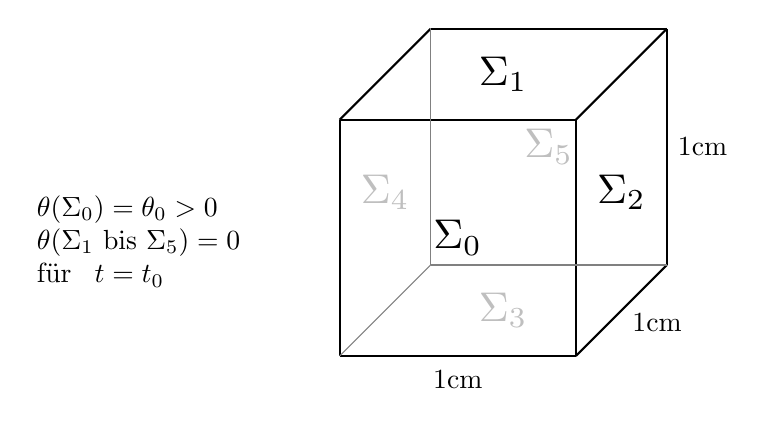
\begin{tikzpicture}
  \newcommand\x{3}
  \newcommand\h{1.5}
  \newcommand\scale{1.5}
  \newcommand\grayton{50}
  \draw[thick](\x,\x,0)--(0,\x,0);
  \draw[thick](0,\x,\x)--(\x,\x,\x);
  \draw[thick](\x,\x,0)--(\x,0,0) node[midway, xshift=3ex]{1cm};
  \draw[thick](\x,0,\x)--(0,0,\x) node[midway, yshift=-2ex]{1cm};
  \draw[thick](\x,\x,\x)--(\x,0,\x);
  \draw[thick](\x,\x,\x)--(\x,0,\x);
  \draw[thick](\x,\x,\x)--(\x,0,\x);
  \draw[thick](\x,\x,\x)--(\x,0,\x);
  \draw[thick](0,\x,\x)--(0,\x,0);  
  \draw[thick](0,\x,\x)--(0,0,\x);
  \draw[thick](\x,\x,0)--(\x,\x,\x);
   \draw[thick](\x,0,0)--(\x,0,\x) node[midway, xshift=3ex, yshift=-1ex]{1cm};
  
  \draw[gray](\x,0,0)--(0,0,0);
  \draw[gray](0,\x,0) -- (0,0,0);
  \draw[gray](0,0,0)--(0,0,\x);
  
  \draw(\h,\h,\x) node[scale=\scale]{$\Sigma_0$};
  \draw(\h,\x,\h) node[scale=\scale]{$\Sigma_1$};
  \draw(\x,\h,\h) node[scale=\scale]{$\Sigma_2$};
  \draw[gray!\grayton](\h,0,\h) node[scale=\scale]{$\Sigma_3$};
  \draw[gray!\grayton](0,\h,\h) node[scale=\scale]{$\Sigma_4$};
  \draw[gray!\grayton](\h,\h,0) node[scale=\scale]{$\Sigma_5$};
  \node[text width=4cm, align=left] at (-3,0.3) {$\theta(\Sigma_0) = \theta_0 > 0$ \\ $\theta(\Sigma_1$ bis $\Sigma_5) = 0$ \\ für \, $t = t_0$};
\end{tikzpicture}
\caption{Die simulierte Geometrie und ihre Anfangsbedeckungsgrade}
\label{fig:cube}
\end{figure}

\paragraph{}
Alle Simulationen wurden in einer Würfelgeometrie, die in der Abbildung~\ref{fig:cube} skizziert ist, durchgeführt. Die Wahl so einer einfachen Geometrie ermöglicht, dass die Ergebnisse im Voraus sehr einfach analytisch berechnet werden können, um sie mit den Simulationsergebnissen zu vergleichen. Die Simulationszeit beträgt 2 Jahre und es werden 1000 Iterationen benutzt. Pro Iteration werden mindestens \SI{e4}{} Testteilchen simuliert. Als der Anfangsbedeckungsgrad der 0. Oberfläche wird der Wert $\theta_0$, der größer als 0 ist, gewählt. Wogegen die Anfangsbedeckungsgrade der anderen Oberflächen als 0 gewählt werden. Es werden die Simulationsergebnisse von drei verschiedenen Anfangswertproblemen gezeigt. Der Anfangsbedeckungsgrad der 0. Oberfläche wird in dem ersten Anfangswertproblem auf 2.0, in dem zweiten Anfangswertproblem auf 3.5 und in dem letzten Anfangswertproblem auf 5.0 gesetzt. Die Temperatur aller Oberflächen beträgt \SI{20}{\celsius}. Außerdem gasen keine Oberflächen aus. Das heißt, die Gesamtteilchenzahl in dem System bleibt erhalten. Folglich wird erwartet, dass der Bedeckungsgrad aller Oberflächen im Gleichgewicht $\frac{\theta_0}{6}$ wird. Für diese Geometrie ist die Wahl eines Anfangsbedeckungsgrads größer als 6.0 nicht zielführend, weil in diesem Fall alle Oberflächen im Gleichgewicht einen Bedeckungsgrad größer als eins haben. Wie am Ende des Abschnitts~\ref{section:implement} erwähnt, führt diese Sache gewissermaßen zum Einfrieren der Simulation. Für die Darstellung der Simulationsergebnisse werden zwei Graphen benutzt. Der erste Graph mit der blauen Kurve zeigt immer den Bedeckungsgrad der 0. Oberfläche, abhängig von der Zeit. Unterdessen ist die Zeitachse logarithmisch skaliert. Der zweite Graph mit der roten Kurve zeigt immer den relativen Fehler (die Abweichung vom Sollwert) im Prozent abhängig von der Zeit. Dabei ist die Zeitachse linear skaliert und es wird ab dem Zeitpunkt, an dem die Simulation konvergiert, betrachtet. Da in den Graphen der relative Fehler betrachtet wird, können die Simulationsergebnisse der Anfangswertprobleme miteinander verglichen werden. Außerdem werden in den Graphen immer die Simulationsergebnisse der 0. Oberfläche gezeigt, denn im Gleichgewicht verhalten sich die anderen Oberflächen analog zur 0. Oberfläche und ihre Simulationsergebnisse zu zeigen wäre unnötig. Letztlich werden die wichtigsten Resultate aus den Simulationen in der Tabelle unter den Graphen dargestellt. Diese Resultate sind die Schrittweite, ab der der relative Fehler 1 \% bzw. 10 \% überschreitet und der maximale relative Fehler. Sie wurden natürlich aus den Simulationsergebnissen aller Oberflächen gesammelt.

\section{Simulationsergebnisse} \label{section:simuergebnisse}
\paragraph{}
Die Abbildung~\ref{fig:figure_2.0}~auf~der~Seite~\pageref{fig:figure_2.0} illustriert die Simulationsergebnisse des vorherigen Verfahrens und der zwei verschiedenen Ansätze des Prädiktor-Korrektor-Verfahrens bei einem Anfangsbedeckungsgrad von 2.0 für die 0. Oberfläche und 0 für die anderen Oberflächen. Im linken Graph ist zu sehen, dass der Bedeckungsgrad in einer kurzen Zeit auf eins fällt. Danach fällt er ziemlich langsam auf den Sollwert. Diese Tatsache ist mit den unterschiedlichen mittleren Verweilzeiten einer Wasser-Wasser-Bindung (\SI{63}{\micro\s}) und einer Wasser-Edelstahl-Bindung (7 Stunden) zu erklären. In allen Simulationen ist das Rauschen ab dem Zeitpunkt von ungefähr \SI{e6}{\s} erkennbar. Hierbei war die Schrittweite ca. 3 Stunden. Daneben ist in den Graphen zu merken und in der Tabelle unter den Graphen zu bestätigen, dass die beiden Ansätze des Prädiktor-Korrektor-Verfahrens das vorherige Verfahren verbessern. Jedoch ist die Verbesserung des ersten Ansatzes vernachlässigbar klein, wogegen die Verbesserung des zweiten Ansatzes bemerkbar ist. Dabei konnte die Schrittweite dreifach erhöht werden, trotzdem blieb der Fehler unter 1 \%. Übrigens ist der maximale Fehler stets unter 5 \%. Die Striche unter dem 10 \% Fehler bedeuten, dass der relative Fehler 10 \% nie überschreitet. Deshalb kann schlussgefolgert werden, dass die Ergebnisse des vorherigen Verfahrens sogar in den größeren Zeitschritten tolerierbar sind. Infolgedessen kann die Anwendung des Prädiktor-Korrektor-Verfahrens verzichtet werden, um Rechenzeit zu sparen.

\paragraph{}
Die Abbildung~\ref{fig:figure_3.5}~auf~der~Seite~\pageref{fig:figure_3.5} stellt die Simulationsergebnisse bei einem Anfangsbedeckungsgrad von 3.5 für die 0. Oberfläche und 0 für die anderen Oberflächen dar. Hier ist deutliche Verbesserung des Prädiktor-Korrektor-Verfahrens gegenüber dem vorherigen Verfahren bemerkbar. Für große Schrittweiten oszillieren die Simulationsergebnisse des vorherigen Verfahrens so stark und dabei entstandener Fehler ist so groß, dass sie nicht mehr akzeptierbar sind. Demgegenüber sind die Ergebnisse der beiden Ansätze des Prädiktor-Korrektor-Verfahrens deutlich besser, wobei der zweite Ansatz noch besser ist. Diese Feststellung kann in der Tabelle unter den Graphen bestätigt werden. Obwohl die Zunahme der Schrittweite, ab der der Fehler 1 \% überschreitet, nicht groß ist, ist sie bei dem 10 \% Fehler deutlich sichtbar. Bei dem zweiten Ansatz überschreitet der Fehler sogar 10 \% nicht und ist stets unter 5 \%. Als Schlussfolgerung kann gesagt werden, dass sich die Anwendung des Prädiktor-Korrektor-Verfahrens für dieses Anfangswertproblem lohnt.

\paragraph{}
Letztlich zeigt die Abbildung~\ref{fig:figure_5.0}~auf~der~Seite~\pageref{fig:figure_5.0} die Simulationsergebnisse bei einem Anfangsbedeckungsgrad von 5.0 für die 0. Oberfläche und 0 für die anderen Oberflächen. In diesem Fall hilft die Anwendung des Prädiktor-Korrektor-Verfahrens nicht viel, weil die Simulationsergebnisse der beiden Ansätze auch oszillieren, wobei sie in dem zweiten Ansatz ein bisschen besser sind, weil der Fehler meistens unter 100 \% bleibt. Außerdem ist die Schrittweite des 10 \% Fehlers bei dem Prädiktor-Korrektor-Verfahren zwar verdoppelt, aber unter Berücksichtigung der verdoppelten Simulationszeit bringt das auch nicht viel. Es kann schlussgefolgert werden, dass in bestimmten Anfangsproblemen sogar das Prädiktor-Korrektor-Verfahren die Oszillation nicht verhindern kann. Die Simulationsergebnisse mit verschiedenen Anfangsbedeckungsgraden zeigen, dass das vorherige Verfahren ab einem Anfangsbedeckungsgrad von 3.0, der erste Ansatz des Prädiktor-Korrektor-Verfahrens ab 4.0 und der zweite Ansatz ab 4.5, wegen der starken Oszillation, unvernünftige Ergebnisse geben. Außerdem wurde festgestellt, dass das Prädiktor-Korrektor-Verfahren mit mehreren Korrektor-Schritten für dieses Anfangswertproblem keine signifikante Verbesserung gegenüber dem Verfahren mit einem Korrektor-Schritt bringt.

%%%%%%%%%%%%%%%%%%%%%%%%%%%%%%%%%%%%%%%%%%%%%%%%%%%%%%%%%%%%%%%%%%%%%%%

\clearpage

\newcommand\ws{0.5}
\begin{figure}[!h]
\centering
\begin{tabular}{@{}cc@{}}
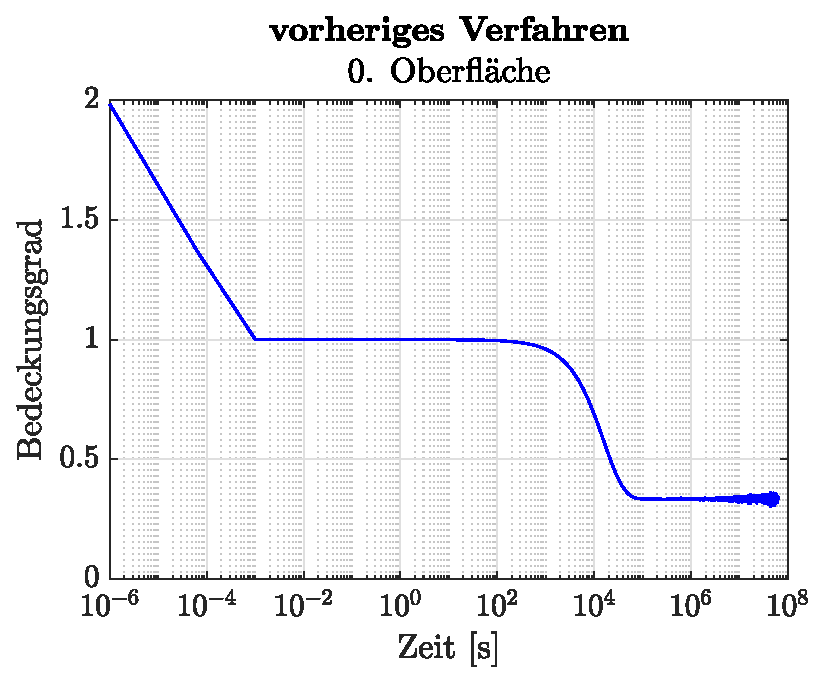
\includegraphics[width=\ws\textwidth]{./include/figure_2.0/old/CovFacet0.eps}&
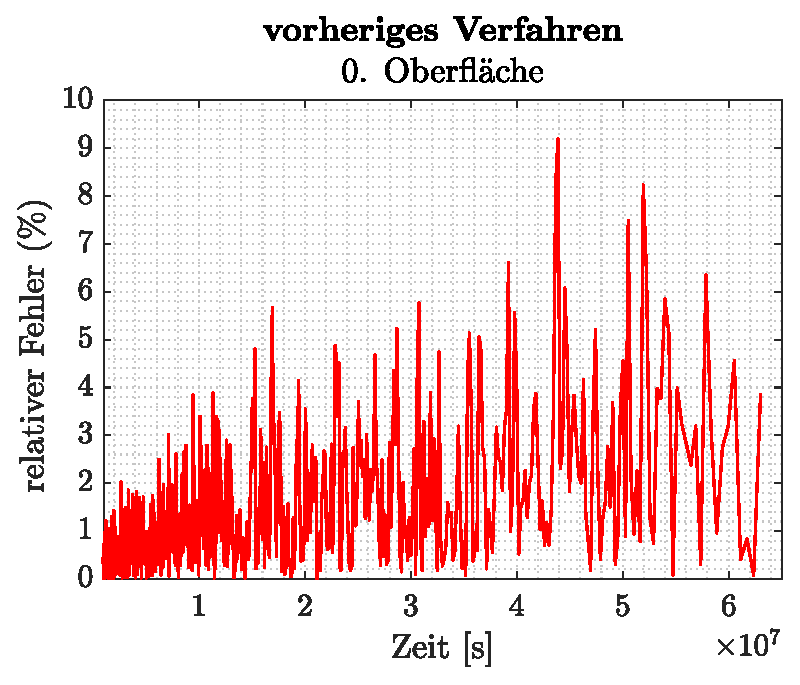
\includegraphics[width=\ws\textwidth]{./include/figure_2.0/old/CovFacetError0.eps}\\
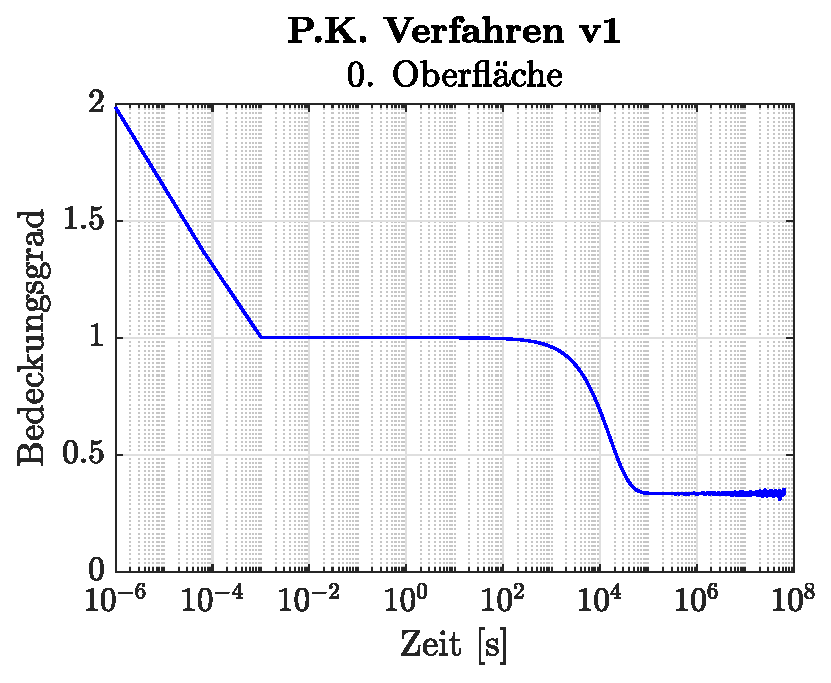
\includegraphics[width=\ws\textwidth]{./include/figure_2.0/PC_current/CovFacet0.eps}&
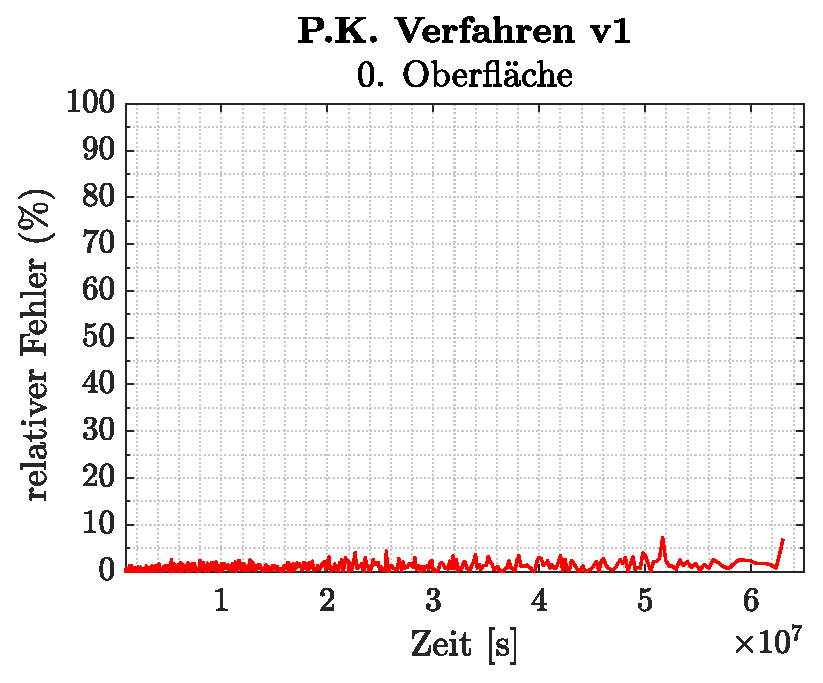
\includegraphics[width=\ws\textwidth]{./include/figure_2.0/PC_current/CovFacetError0.eps}\\
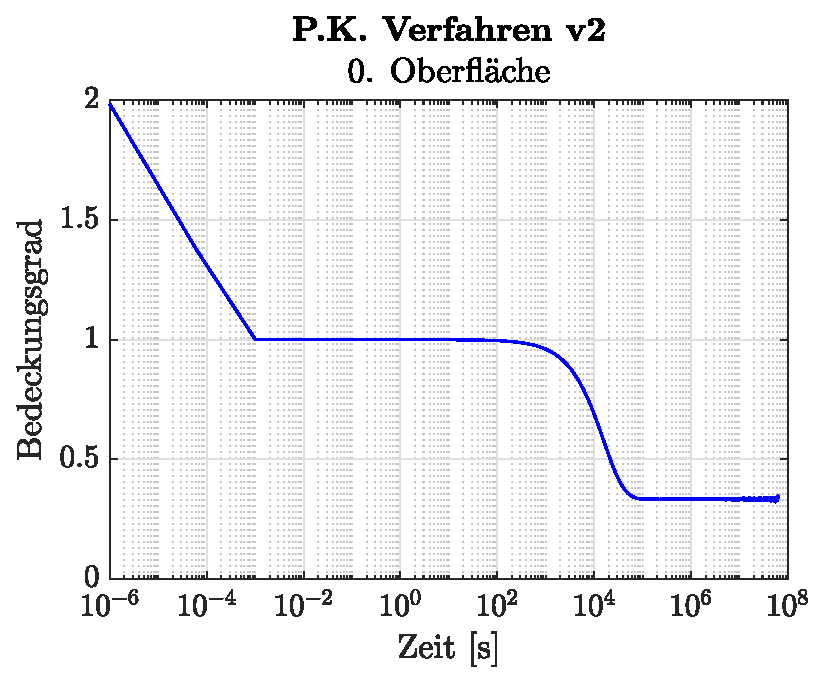
\includegraphics[width=\ws\textwidth]{./include/figure_2.0/PC_new/CovFacet0.eps}&
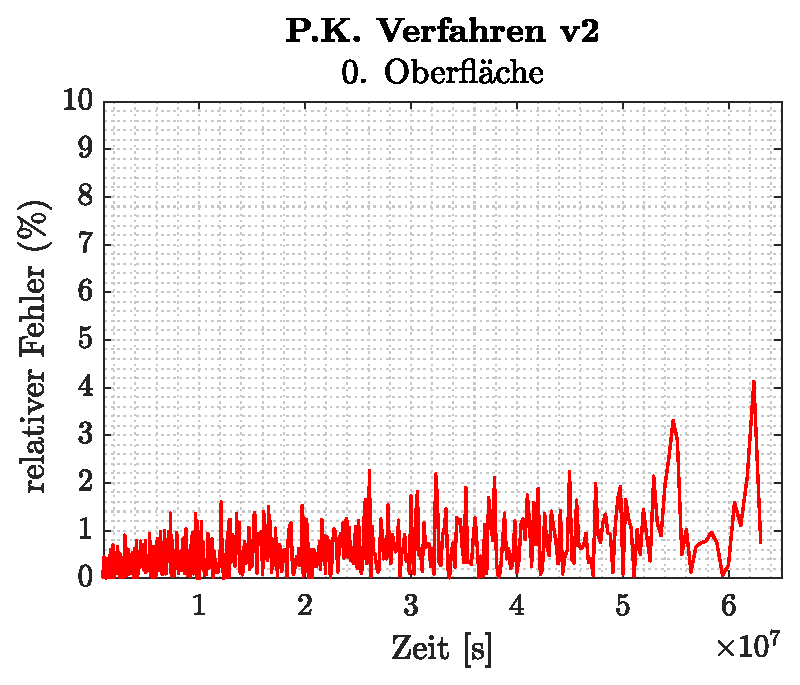
\includegraphics[width=\ws\textwidth]{./include/figure_2.0/PC_new/CovFacetError0.eps}
\end{tabular}
\newline
\vspace*{0.5cm}
\newline
\begin{tabular}{|c|c|c|c|}
\hline
$\theta_0 = 2.0$ & 1 \% Fehler & 10 \% Fehler & Max. rel. Fehler\\
\hline
Vorheriges Verfahren & 7735 s & -- & 9.53 \% \\
P.K. Verfahren v1 & 12780 s & -- & 8.24 \% \\
P.K. Verfahren v2 & 23330 s & -- & 4.70 \% \\
\hline
\end{tabular}
\caption{Simulationsergebnisse für $\theta_0 = 2.0$}
\label{fig:figure_2.0}
\end{figure}

%%%%%%%%%%%%%%%%%%%%%%%%%%%%%%%%%%%%%%%%%%%%%%%%%%%%%%%%%%%%%%%%%%%%%%%

\clearpage
\newcommand\wss{0.5}
\begin{figure}[!h]
\centering
\begin{tabular}{@{}cc@{}}
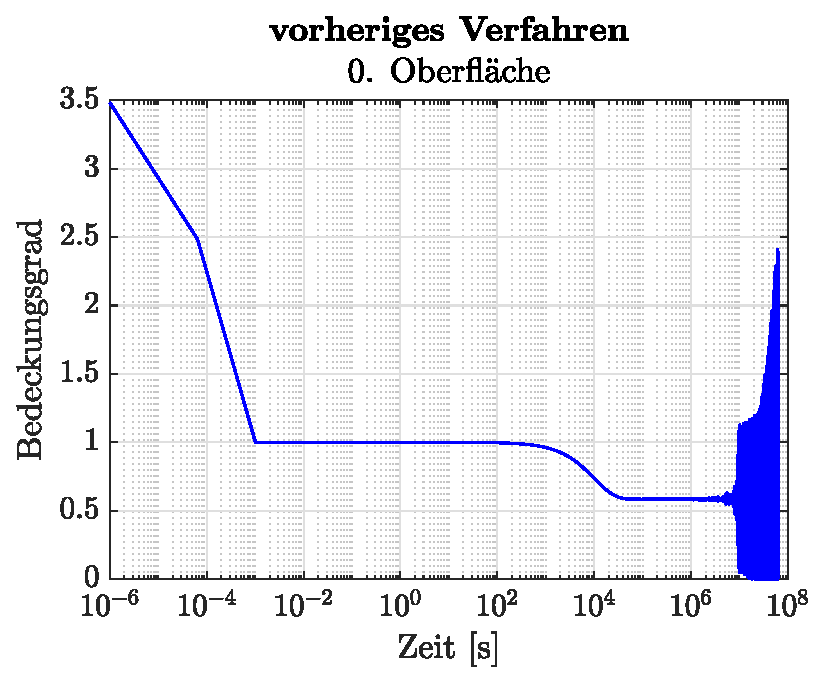
\includegraphics[width=\wss\textwidth]{./include/figure_3.5/old/CovFacet0.eps}&
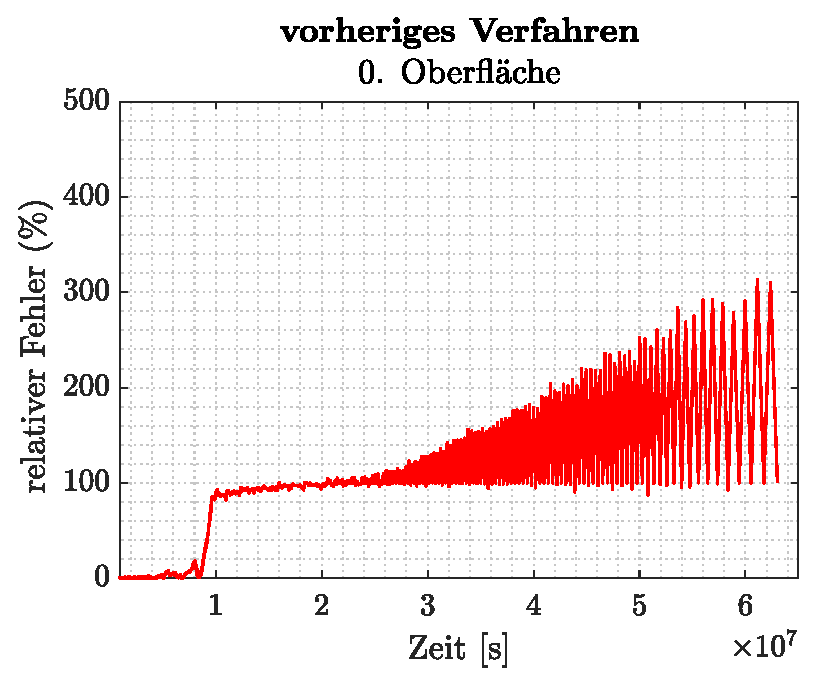
\includegraphics[width=\wss\textwidth]{./include/figure_3.5/old/CovFacetError0.eps}\\
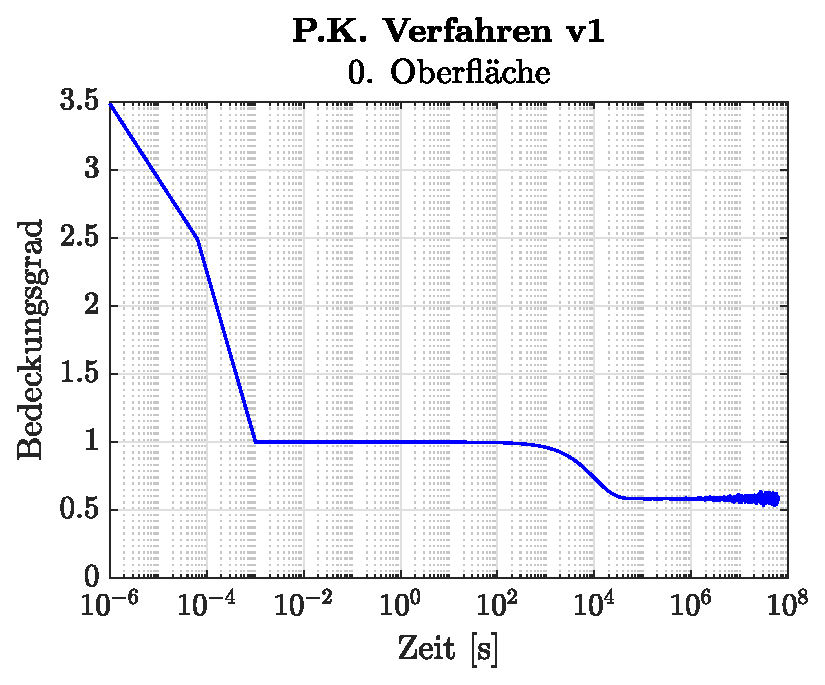
\includegraphics[width=\wss\textwidth]{./include/figure_3.5/PC_current/CovFacet0.eps}&
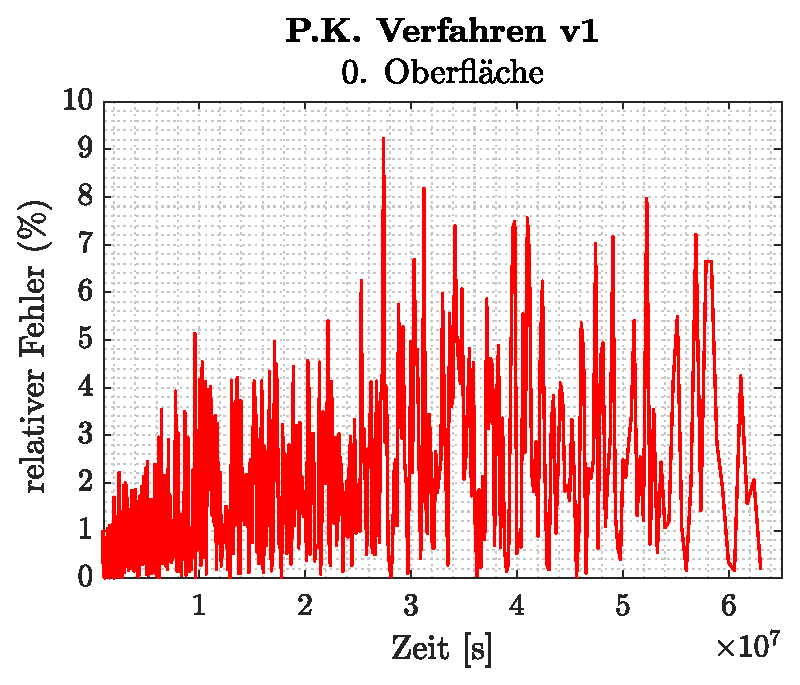
\includegraphics[width=\wss\textwidth]{./include/figure_3.5/PC_current/CovFacetError0.eps}\\
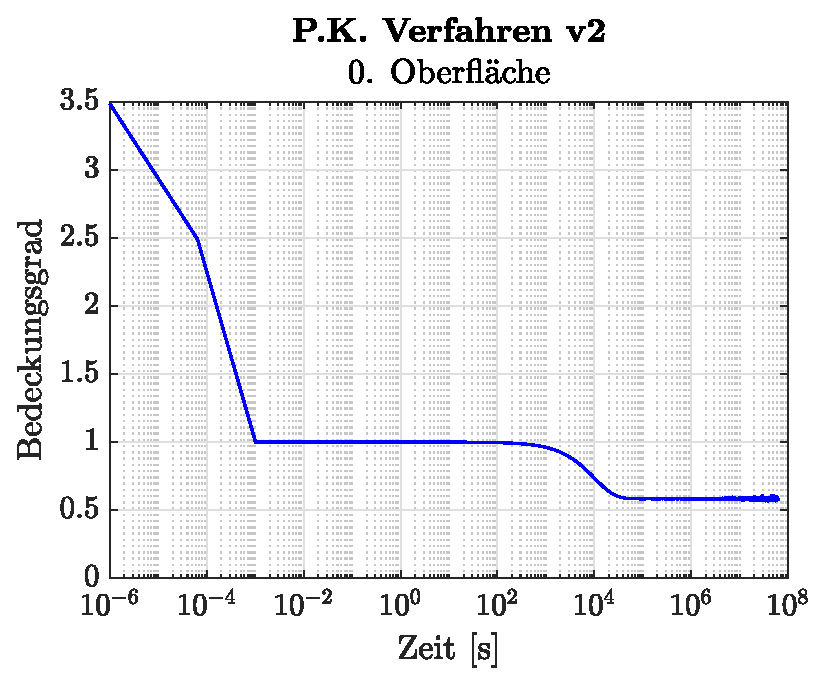
\includegraphics[width=\wss\textwidth]{./include/figure_3.5/PC_new/CovFacet0.eps}&
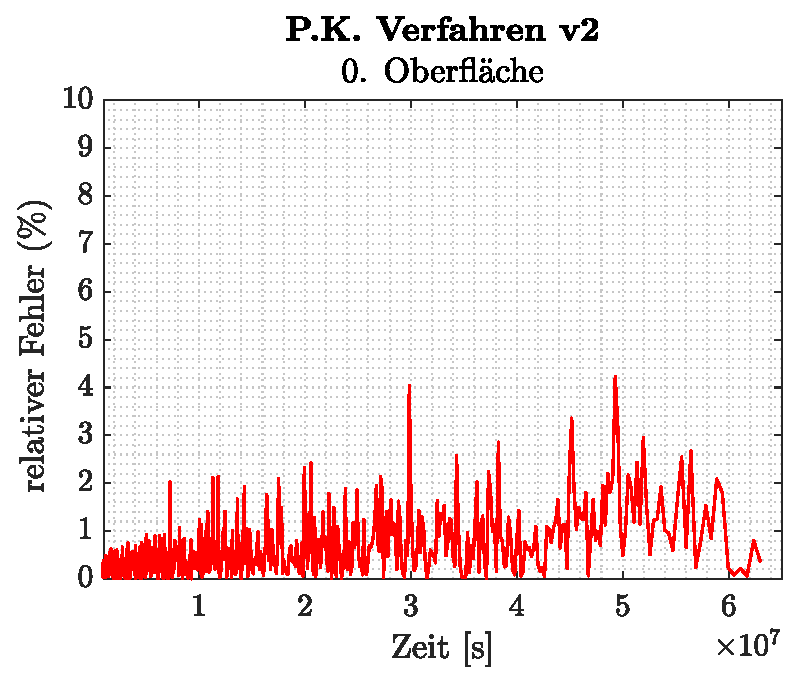
\includegraphics[width=\wss\textwidth]{./include/figure_3.5/PC_new/CovFacetError0.eps}
\end{tabular}
\newline
\vspace*{0.5cm}
\newline
\begin{tabular}{|c|c|c|c|}
\hline
$\theta_0 = 3.5$ & 1 \% Fehler & 10 \% Fehler & Max. rel. Fehler\\
\hline
Vorheriges Verfahren & 10007 s & 44870 s & 316.41 \% \\
P.K. Verfahren v1 & 7017 s & 165900 s & 11.98 \% \\
P.K. Verfahren v2 & 29730 s & -- & 4.23 \% \\
\hline
\end{tabular}
\caption{Simulationsergebnisse für $\theta_0 = 3.5$}
\label{fig:figure_3.5}
\end{figure}

%%%%%%%%%%%%%%%%%%%%%%%%%%%%%%%%%%%%%%%%%%%%%%%%%%%%%%%%%%%%%%%%%%%%%%%

\clearpage
\newcommand\wsss{0.5}
\begin{figure}[!h]
\centering
\begin{tabular}{@{}cc@{}}
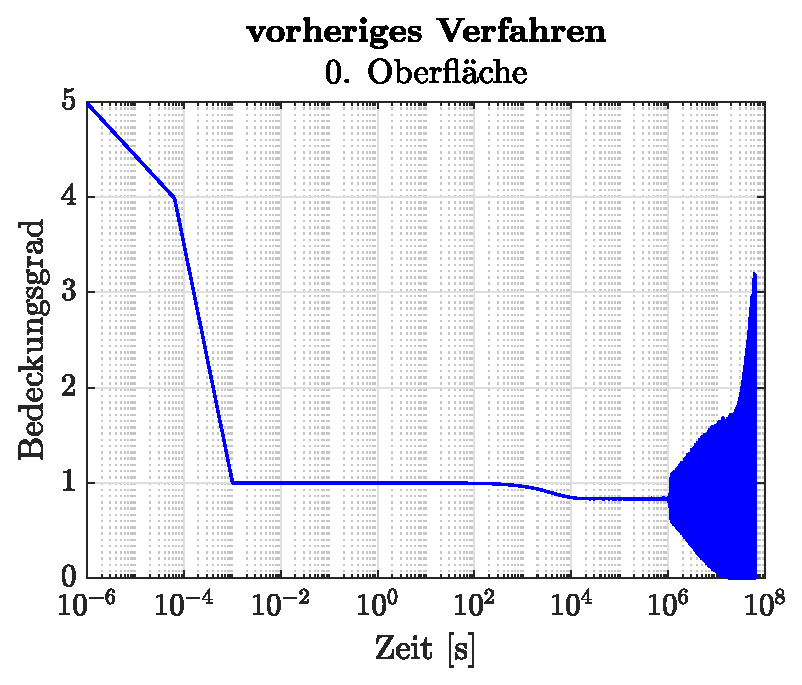
\includegraphics[width=\wsss\textwidth]{./include/figure_5.0/old/CovFacet0.eps}&
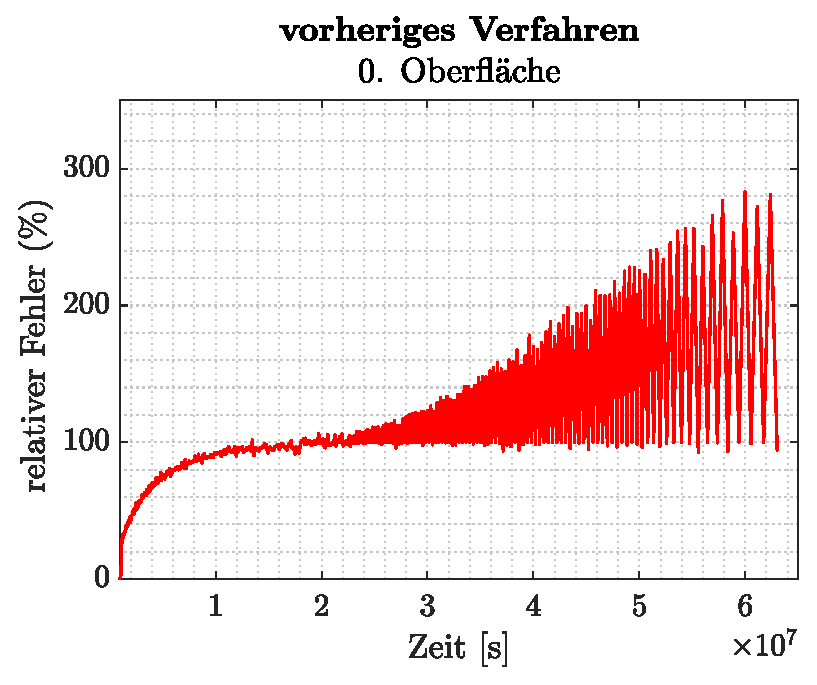
\includegraphics[width=\wsss\textwidth]{./include/figure_5.0/old/CovFacetError0.eps}\\
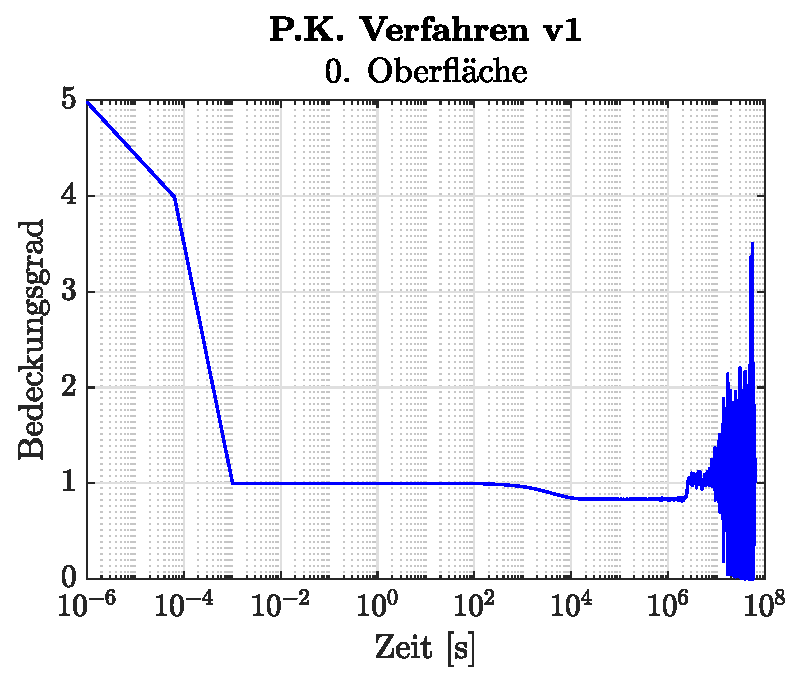
\includegraphics[width=\wsss\textwidth]{./include/figure_5.0/PC_current/CovFacet0.eps}&
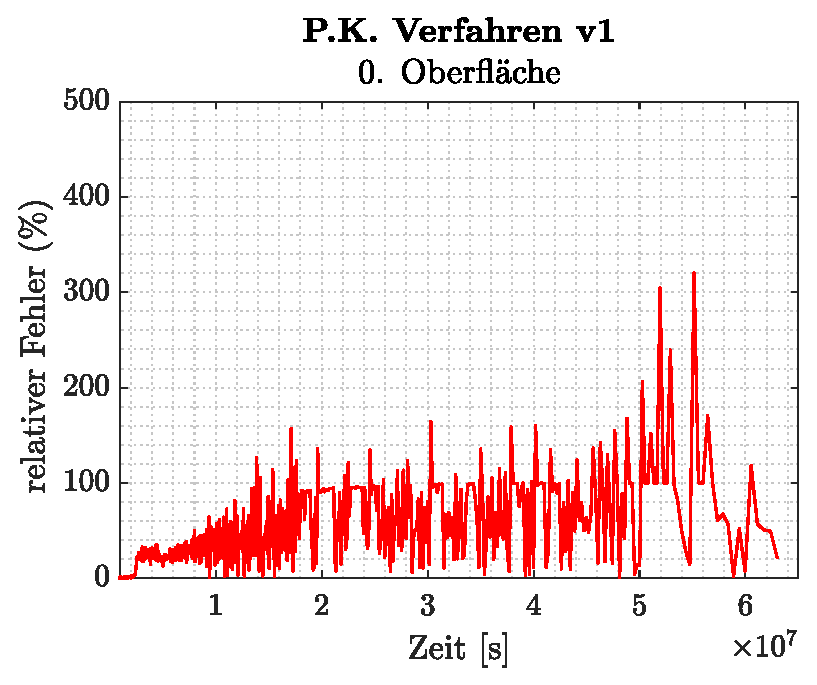
\includegraphics[width=\wsss\textwidth]{./include/figure_5.0/PC_current/CovFacetError0.eps}\\
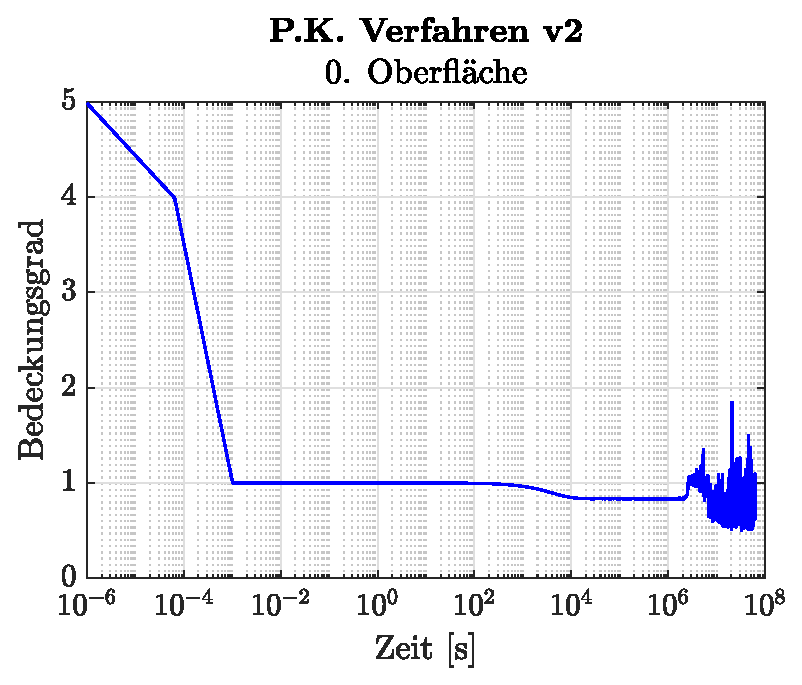
\includegraphics[width=\wsss\textwidth]{./include/figure_5.0/PC_new/CovFacet0.eps}&
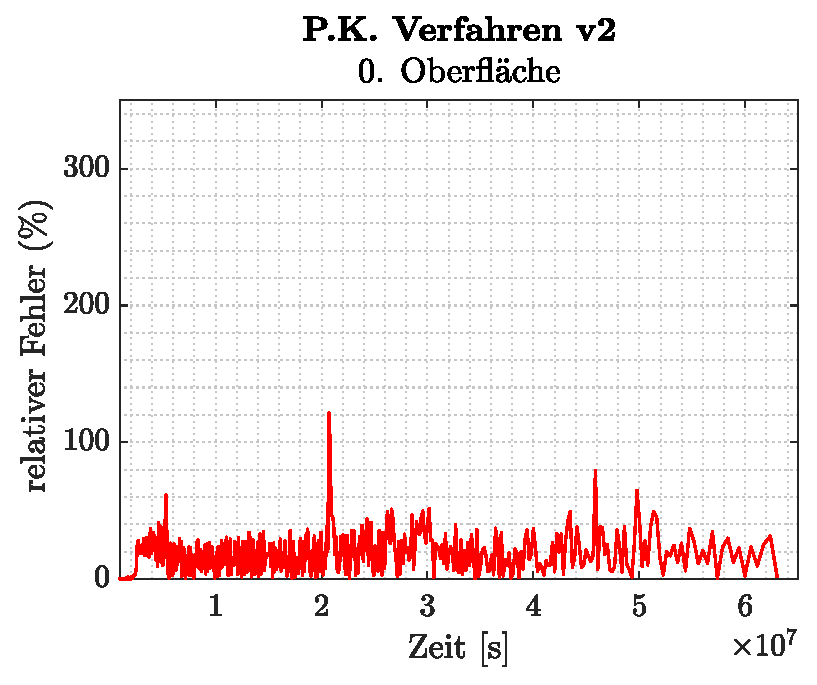
\includegraphics[width=\wsss\textwidth]{./include/figure_5.0/PC_new/CovFacetError0.eps}
\end{tabular}
\newline
\vspace*{0.5cm}
\newline
\begin{tabular}{|c|c|c|c|}
\hline
$\theta_0 = 5.0$ & 1 \% Fehler & 10 \% Fehler & Max. rel. Fehler\\
\hline
Vorheriges Verfahren & 7885 s & 10821 s & 291.05 \% \\
P.K. Verfahren v1 & 8985 s & 21220 s & 403.05 \% \\
P.K. Verfahren v2 & 13860 s & 22560 s & 174.84 \% \\
\hline
\end{tabular}
\caption{Simulationsergebnisse für $\theta_0 = 5.0$}
\label{fig:figure_5.0}
\end{figure}

%%%%%%%%%%%%%%%%%%%%%%%%%%%%%%%%%%%%%%%%%%%%%%%%%%%%%%%%%%%%%%%%%%%%%%%

\chapter{Abschluss und Ausblick} \label{chap:abschluss}
\paragraph{}
In dieser Ingenieurpraxis wurde die Implementierung des Prädiktor-Korrektor-Verfahrens in dem Programm „ContaminationFlow“ für die Berechnung der Bedeckung erklärt. Dazu wurde hauptsächlich auf zwei verschiedenen Implementierungsansätzen eingegangen. Die Simulationsergebnisse zeigten, dass das Prädiktor-Korrektor-Verfahren für manche Anfangswertprobleme eine deutliche Verbesserung im Vergleich zu dem vorherigen Verfahren bringt. Jedoch gibt es auch die Anfangswertprobleme, für die die Anwendung des neuen Verfahrens nicht viel bringt. In Kapitel~\ref{chap:auswertung} wurde gezeigt, dass die Anwendung des Prädiktor-Korrektor-Verfahrens in einer Würfelgeometrie mit den Anfangsbedeckungsgraden von 2.0 und 5.0 für die 0. Oberfläche und 0 für die anderen Oberflächen, nicht unbedingt nötig war, weil das vorherige Verfahren entweder tolerierbare Ergebnisse gab oder das neue Verfahren das Oszillationsproblem nicht lösen konnte. Es wurde festgestellt, dass das Prädiktor-Korrektor-Verfahren keinen Vorteil mehr bringt, wenn die Bedeckungsgrade der Oberflächen sich im Gleichgewicht auf eins annähren. Aus diesem Grund wurde die Anwendung des Verfahrens in der Simulation optional gewählt. Die beiden Ansätze des Prädiktor-Korrektor-Verfahrens wurden gegenübergestellt. Dabei wurde es festgestellt, dass der zweite Ansatz, in dem das Prinzip des Heunverfahrens direkt in den Code eingebaut wird, tatsächlich besser als der erste Ansatz funktioniert. Nichtsdestotrotz kann es in dem zweiten Ansatz vorkommen, dass die Simulation einfriert, weil die Simulationsergebnisse so oszillieren, dass alle Oberflächen plötzlich über einen Bedeckungsgrad von mehr als eins verfügen. Das Auftreten dieses Problems ist doch sehr unwahrscheinlich und kann mit der Erhöhung der Anzahl der simulierten Teilchen gelöst werden.
%\paragraph{}
Als Ausblick empfehle ich, dass das Prädiktor-Korrektor-Verfahren und das vorherige Verfahren nicht in einer sehr einfachen Würfelgeometrie, sondern in einer komplexeren Geometrie verglichen werden soll. Folglich kann deduziert werden, ob das Verfahren bei einer realistischeren Simulation immer noch einen Vorteil gegenüber dem vorherigen Verfahren bringt. Da die Simulation in einer komplexeren Geometrie ausgeführt wird, wäre es nicht einfach, die Sollwerte der Bedeckungen vorweg zu wissen, bzw. analytisch zu berechnen. Demnach wäre es vernünftig, dass die gleiche Geometrie in einem realen Experiment beobachtet wird und dabei möglichst viele 	Messwerte gesammelt wird. Außerdem kann es sein, dass die Anwendung eines Algorithmus, der zur numerischen Lösung einer Differenzialgleichung entwickelt wurde, nicht zielführend in einer ereignisgesteuerten Simulation ist. Aus diesem Grund soll der Algorithmus eventuell für die ereignisgesteuerten Simulationen angepasst werden.


% --- Bibliography
\cleardoublepage
\bibliographystyle{unsrturl}
\bibliography{bericht}

% --- Mandatory confirmation.
\confirmation

\end{document}

%%% Local Variables:
%%% mode: latex
%%% TeX-master: t
%%% End:
